% Options for packages loaded elsewhere
\PassOptionsToPackage{unicode}{hyperref}
\PassOptionsToPackage{hyphens}{url}
\PassOptionsToPackage{dvipsnames,svgnames,x11names}{xcolor}
%
\documentclass[
  letterpaper,
  DIV=11,
  numbers=noendperiod]{scrartcl}

\usepackage{amsmath,amssymb}
\usepackage{iftex}
\ifPDFTeX
  \usepackage[T1]{fontenc}
  \usepackage[utf8]{inputenc}
  \usepackage{textcomp} % provide euro and other symbols
\else % if luatex or xetex
  \usepackage{unicode-math}
  \defaultfontfeatures{Scale=MatchLowercase}
  \defaultfontfeatures[\rmfamily]{Ligatures=TeX,Scale=1}
\fi
\usepackage{lmodern}
\ifPDFTeX\else  
    % xetex/luatex font selection
\fi
% Use upquote if available, for straight quotes in verbatim environments
\IfFileExists{upquote.sty}{\usepackage{upquote}}{}
\IfFileExists{microtype.sty}{% use microtype if available
  \usepackage[]{microtype}
  \UseMicrotypeSet[protrusion]{basicmath} % disable protrusion for tt fonts
}{}
\makeatletter
\@ifundefined{KOMAClassName}{% if non-KOMA class
  \IfFileExists{parskip.sty}{%
    \usepackage{parskip}
  }{% else
    \setlength{\parindent}{0pt}
    \setlength{\parskip}{6pt plus 2pt minus 1pt}}
}{% if KOMA class
  \KOMAoptions{parskip=half}}
\makeatother
\usepackage{xcolor}
\setlength{\emergencystretch}{3em} % prevent overfull lines
\setcounter{secnumdepth}{-\maxdimen} % remove section numbering
% Make \paragraph and \subparagraph free-standing
\makeatletter
\ifx\paragraph\undefined\else
  \let\oldparagraph\paragraph
  \renewcommand{\paragraph}{
    \@ifstar
      \xxxParagraphStar
      \xxxParagraphNoStar
  }
  \newcommand{\xxxParagraphStar}[1]{\oldparagraph*{#1}\mbox{}}
  \newcommand{\xxxParagraphNoStar}[1]{\oldparagraph{#1}\mbox{}}
\fi
\ifx\subparagraph\undefined\else
  \let\oldsubparagraph\subparagraph
  \renewcommand{\subparagraph}{
    \@ifstar
      \xxxSubParagraphStar
      \xxxSubParagraphNoStar
  }
  \newcommand{\xxxSubParagraphStar}[1]{\oldsubparagraph*{#1}\mbox{}}
  \newcommand{\xxxSubParagraphNoStar}[1]{\oldsubparagraph{#1}\mbox{}}
\fi
\makeatother

\usepackage{color}
\usepackage{fancyvrb}
\newcommand{\VerbBar}{|}
\newcommand{\VERB}{\Verb[commandchars=\\\{\}]}
\DefineVerbatimEnvironment{Highlighting}{Verbatim}{commandchars=\\\{\}}
% Add ',fontsize=\small' for more characters per line
\usepackage{framed}
\definecolor{shadecolor}{RGB}{241,243,245}
\newenvironment{Shaded}{\begin{snugshade}}{\end{snugshade}}
\newcommand{\AlertTok}[1]{\textcolor[rgb]{0.68,0.00,0.00}{#1}}
\newcommand{\AnnotationTok}[1]{\textcolor[rgb]{0.37,0.37,0.37}{#1}}
\newcommand{\AttributeTok}[1]{\textcolor[rgb]{0.40,0.45,0.13}{#1}}
\newcommand{\BaseNTok}[1]{\textcolor[rgb]{0.68,0.00,0.00}{#1}}
\newcommand{\BuiltInTok}[1]{\textcolor[rgb]{0.00,0.23,0.31}{#1}}
\newcommand{\CharTok}[1]{\textcolor[rgb]{0.13,0.47,0.30}{#1}}
\newcommand{\CommentTok}[1]{\textcolor[rgb]{0.37,0.37,0.37}{#1}}
\newcommand{\CommentVarTok}[1]{\textcolor[rgb]{0.37,0.37,0.37}{\textit{#1}}}
\newcommand{\ConstantTok}[1]{\textcolor[rgb]{0.56,0.35,0.01}{#1}}
\newcommand{\ControlFlowTok}[1]{\textcolor[rgb]{0.00,0.23,0.31}{\textbf{#1}}}
\newcommand{\DataTypeTok}[1]{\textcolor[rgb]{0.68,0.00,0.00}{#1}}
\newcommand{\DecValTok}[1]{\textcolor[rgb]{0.68,0.00,0.00}{#1}}
\newcommand{\DocumentationTok}[1]{\textcolor[rgb]{0.37,0.37,0.37}{\textit{#1}}}
\newcommand{\ErrorTok}[1]{\textcolor[rgb]{0.68,0.00,0.00}{#1}}
\newcommand{\ExtensionTok}[1]{\textcolor[rgb]{0.00,0.23,0.31}{#1}}
\newcommand{\FloatTok}[1]{\textcolor[rgb]{0.68,0.00,0.00}{#1}}
\newcommand{\FunctionTok}[1]{\textcolor[rgb]{0.28,0.35,0.67}{#1}}
\newcommand{\ImportTok}[1]{\textcolor[rgb]{0.00,0.46,0.62}{#1}}
\newcommand{\InformationTok}[1]{\textcolor[rgb]{0.37,0.37,0.37}{#1}}
\newcommand{\KeywordTok}[1]{\textcolor[rgb]{0.00,0.23,0.31}{\textbf{#1}}}
\newcommand{\NormalTok}[1]{\textcolor[rgb]{0.00,0.23,0.31}{#1}}
\newcommand{\OperatorTok}[1]{\textcolor[rgb]{0.37,0.37,0.37}{#1}}
\newcommand{\OtherTok}[1]{\textcolor[rgb]{0.00,0.23,0.31}{#1}}
\newcommand{\PreprocessorTok}[1]{\textcolor[rgb]{0.68,0.00,0.00}{#1}}
\newcommand{\RegionMarkerTok}[1]{\textcolor[rgb]{0.00,0.23,0.31}{#1}}
\newcommand{\SpecialCharTok}[1]{\textcolor[rgb]{0.37,0.37,0.37}{#1}}
\newcommand{\SpecialStringTok}[1]{\textcolor[rgb]{0.13,0.47,0.30}{#1}}
\newcommand{\StringTok}[1]{\textcolor[rgb]{0.13,0.47,0.30}{#1}}
\newcommand{\VariableTok}[1]{\textcolor[rgb]{0.07,0.07,0.07}{#1}}
\newcommand{\VerbatimStringTok}[1]{\textcolor[rgb]{0.13,0.47,0.30}{#1}}
\newcommand{\WarningTok}[1]{\textcolor[rgb]{0.37,0.37,0.37}{\textit{#1}}}

\providecommand{\tightlist}{%
  \setlength{\itemsep}{0pt}\setlength{\parskip}{0pt}}\usepackage{longtable,booktabs,array}
\usepackage{calc} % for calculating minipage widths
% Correct order of tables after \paragraph or \subparagraph
\usepackage{etoolbox}
\makeatletter
\patchcmd\longtable{\par}{\if@noskipsec\mbox{}\fi\par}{}{}
\makeatother
% Allow footnotes in longtable head/foot
\IfFileExists{footnotehyper.sty}{\usepackage{footnotehyper}}{\usepackage{footnote}}
\makesavenoteenv{longtable}
\usepackage{graphicx}
\makeatletter
\newsavebox\pandoc@box
\newcommand*\pandocbounded[1]{% scales image to fit in text height/width
  \sbox\pandoc@box{#1}%
  \Gscale@div\@tempa{\textheight}{\dimexpr\ht\pandoc@box+\dp\pandoc@box\relax}%
  \Gscale@div\@tempb{\linewidth}{\wd\pandoc@box}%
  \ifdim\@tempb\p@<\@tempa\p@\let\@tempa\@tempb\fi% select the smaller of both
  \ifdim\@tempa\p@<\p@\scalebox{\@tempa}{\usebox\pandoc@box}%
  \else\usebox{\pandoc@box}%
  \fi%
}
% Set default figure placement to htbp
\def\fps@figure{htbp}
\makeatother

\usepackage{fvextra}
\DefineVerbatimEnvironment{Highlighting}{Verbatim}{breaklines,commandchars=\\\{\}}
\DefineVerbatimEnvironment{OutputCode}{Verbatim}{breaklines,commandchars=\\\{\}}
\KOMAoption{captions}{tableheading}
\makeatletter
\@ifpackageloaded{caption}{}{\usepackage{caption}}
\AtBeginDocument{%
\ifdefined\contentsname
  \renewcommand*\contentsname{Table of contents}
\else
  \newcommand\contentsname{Table of contents}
\fi
\ifdefined\listfigurename
  \renewcommand*\listfigurename{List of Figures}
\else
  \newcommand\listfigurename{List of Figures}
\fi
\ifdefined\listtablename
  \renewcommand*\listtablename{List of Tables}
\else
  \newcommand\listtablename{List of Tables}
\fi
\ifdefined\figurename
  \renewcommand*\figurename{Figure}
\else
  \newcommand\figurename{Figure}
\fi
\ifdefined\tablename
  \renewcommand*\tablename{Table}
\else
  \newcommand\tablename{Table}
\fi
}
\@ifpackageloaded{float}{}{\usepackage{float}}
\floatstyle{ruled}
\@ifundefined{c@chapter}{\newfloat{codelisting}{h}{lop}}{\newfloat{codelisting}{h}{lop}[chapter]}
\floatname{codelisting}{Listing}
\newcommand*\listoflistings{\listof{codelisting}{List of Listings}}
\makeatother
\makeatletter
\makeatother
\makeatletter
\@ifpackageloaded{caption}{}{\usepackage{caption}}
\@ifpackageloaded{subcaption}{}{\usepackage{subcaption}}
\makeatother

\usepackage{bookmark}

\IfFileExists{xurl.sty}{\usepackage{xurl}}{} % add URL line breaks if available
\urlstyle{same} % disable monospaced font for URLs
\hypersetup{
  pdftitle={IMC round 1},
  colorlinks=true,
  linkcolor={blue},
  filecolor={Maroon},
  citecolor={Blue},
  urlcolor={Blue},
  pdfcreator={LaTeX via pandoc}}


\title{IMC round 1}
\author{}
\date{}

\begin{document}
\maketitle


\begin{Shaded}
\begin{Highlighting}[]
\ImportTok{import}\NormalTok{ pandas }\ImportTok{as}\NormalTok{ pd}
\ImportTok{import}\NormalTok{ numpy }\ImportTok{as}\NormalTok{ np}
\ImportTok{import}\NormalTok{ os}
\ImportTok{import}\NormalTok{ sys}
\end{Highlighting}
\end{Shaded}

\begin{Shaded}
\begin{Highlighting}[]
\NormalTok{df1 }\OperatorTok{=}\NormalTok{ pd.read\_csv(}\StringTok{\textquotesingle{}round{-}1{-}island{-}data{-}bottle/round{-}1{-}island{-}data{-}bottle/prices\_round\_1\_day\_{-}2.csv\textquotesingle{}}\NormalTok{,sep}\OperatorTok{=}\StringTok{\textquotesingle{};\textquotesingle{}}\NormalTok{)}
\NormalTok{df2 }\OperatorTok{=}\NormalTok{ pd.read\_csv(}\StringTok{\textquotesingle{}round{-}1{-}island{-}data{-}bottle/round{-}1{-}island{-}data{-}bottle/prices\_round\_1\_day\_{-}1.csv\textquotesingle{}}\NormalTok{,sep}\OperatorTok{=}\StringTok{\textquotesingle{};\textquotesingle{}}\NormalTok{)}
\NormalTok{df3 }\OperatorTok{=}\NormalTok{ pd.read\_csv(}\StringTok{\textquotesingle{}round{-}1{-}island{-}data{-}bottle/round{-}1{-}island{-}data{-}bottle/prices\_round\_1\_day\_0.csv\textquotesingle{}}\NormalTok{,sep}\OperatorTok{=}\StringTok{\textquotesingle{};\textquotesingle{}}\NormalTok{)}
\end{Highlighting}
\end{Shaded}

\begin{Shaded}
\begin{Highlighting}[]
\NormalTok{df\_squid }\OperatorTok{=}\NormalTok{ pd.concat([df1[df1[}\StringTok{\textquotesingle{}product\textquotesingle{}}\NormalTok{] }\OperatorTok{==} \StringTok{\textquotesingle{}SQUID\_INK\textquotesingle{}}\NormalTok{],df2[df2[}\StringTok{\textquotesingle{}product\textquotesingle{}}\NormalTok{] }\OperatorTok{==} \StringTok{\textquotesingle{}SQUID\_INK\textquotesingle{}}\NormalTok{],df3[df3[}\StringTok{\textquotesingle{}product\textquotesingle{}}\NormalTok{] }\OperatorTok{==} \StringTok{\textquotesingle{}SQUID\_INK\textquotesingle{}}\NormalTok{]]).reset\_index(drop}\OperatorTok{=}\VariableTok{True}\NormalTok{)}
\NormalTok{df\_kelp }\OperatorTok{=}\NormalTok{ pd.concat([df1[df1[}\StringTok{\textquotesingle{}product\textquotesingle{}}\NormalTok{] }\OperatorTok{==} \StringTok{\textquotesingle{}KELP\textquotesingle{}}\NormalTok{],df2[df2[}\StringTok{\textquotesingle{}product\textquotesingle{}}\NormalTok{] }\OperatorTok{==} \StringTok{\textquotesingle{}KELP\textquotesingle{}}\NormalTok{],df3[df3[}\StringTok{\textquotesingle{}product\textquotesingle{}}\NormalTok{] }\OperatorTok{==} \StringTok{\textquotesingle{}KELP\textquotesingle{}}\NormalTok{]]).reset\_index(drop}\OperatorTok{=}\VariableTok{True}\NormalTok{)}
\end{Highlighting}
\end{Shaded}

\begin{Shaded}
\begin{Highlighting}[]
\NormalTok{df\_m }\OperatorTok{=}\NormalTok{ pd.merge(df\_squid[[}\StringTok{\textquotesingle{}day\textquotesingle{}}\NormalTok{,}\StringTok{\textquotesingle{}timestamp\textquotesingle{}}\NormalTok{,}\StringTok{\textquotesingle{}mid\_price\textquotesingle{}}\NormalTok{]].rename(columns}\OperatorTok{=}\NormalTok{\{}\StringTok{\textquotesingle{}mid\_price\textquotesingle{}}\NormalTok{:}\StringTok{\textquotesingle{}squid\_mid\_price\textquotesingle{}}\NormalTok{\}),df\_kelp[[}\StringTok{\textquotesingle{}day\textquotesingle{}}\NormalTok{,}\StringTok{\textquotesingle{}timestamp\textquotesingle{}}\NormalTok{,}\StringTok{\textquotesingle{}mid\_price\textquotesingle{}}\NormalTok{]].rename(columns}\OperatorTok{=}\NormalTok{\{}\StringTok{\textquotesingle{}mid\_price\textquotesingle{}}\NormalTok{:}\StringTok{\textquotesingle{}kelp\_mid\_price\textquotesingle{}}\NormalTok{\}),on}\OperatorTok{=}\NormalTok{[}\StringTok{\textquotesingle{}day\textquotesingle{}}\NormalTok{,}\StringTok{\textquotesingle{}timestamp\textquotesingle{}}\NormalTok{],how}\OperatorTok{=}\StringTok{\textquotesingle{}outer\textquotesingle{}}\NormalTok{)}
\end{Highlighting}
\end{Shaded}

\begin{Shaded}
\begin{Highlighting}[]
\NormalTok{df\_m[}\StringTok{\textquotesingle{}squid\_mid\_price\_ytd\textquotesingle{}}\NormalTok{] }\OperatorTok{=}\NormalTok{ df\_m[}\StringTok{\textquotesingle{}squid\_mid\_price\textquotesingle{}}\NormalTok{].shift(}\DecValTok{1}\NormalTok{)}
\NormalTok{df\_m[}\StringTok{\textquotesingle{}kelp\_mid\_price\_ytd\textquotesingle{}}\NormalTok{] }\OperatorTok{=}\NormalTok{ df\_m[}\StringTok{\textquotesingle{}kelp\_mid\_price\textquotesingle{}}\NormalTok{].shift(}\DecValTok{1}\NormalTok{)}
\end{Highlighting}
\end{Shaded}

\begin{Shaded}
\begin{Highlighting}[]
\NormalTok{df\_m[}\StringTok{\textquotesingle{}squid\_mid\_ret\textquotesingle{}}\NormalTok{] }\OperatorTok{=}\NormalTok{ df\_m[}\StringTok{\textquotesingle{}squid\_mid\_price\textquotesingle{}}\NormalTok{].pct\_change()}
\NormalTok{df\_m[}\StringTok{\textquotesingle{}kelp\_mid\_ret\textquotesingle{}}\NormalTok{] }\OperatorTok{=}\NormalTok{ df\_m[}\StringTok{\textquotesingle{}kelp\_mid\_price\textquotesingle{}}\NormalTok{].pct\_change()}
\NormalTok{df\_m[}\StringTok{\textquotesingle{}squid\_mid\_ret\_ytd\textquotesingle{}}\NormalTok{] }\OperatorTok{=}\NormalTok{ df\_m[}\StringTok{\textquotesingle{}squid\_mid\_ret\textquotesingle{}}\NormalTok{].shift(}\DecValTok{1}\NormalTok{)}
\NormalTok{df\_m[}\StringTok{\textquotesingle{}kelp\_mid\_ret\_ytd\textquotesingle{}}\NormalTok{] }\OperatorTok{=}\NormalTok{ df\_m[}\StringTok{\textquotesingle{}kelp\_mid\_ret\textquotesingle{}}\NormalTok{].shift(}\DecValTok{1}\NormalTok{)}
\end{Highlighting}
\end{Shaded}

\begin{Shaded}
\begin{Highlighting}[]
\ImportTok{import}\NormalTok{ klib }\ImportTok{as}\NormalTok{ kl}
\end{Highlighting}
\end{Shaded}

\begin{Shaded}
\begin{Highlighting}[]
\NormalTok{kl.corr\_plot(df\_m[[}\StringTok{\textquotesingle{}squid\_mid\_ret\_ytd\textquotesingle{}}\NormalTok{,}\StringTok{\textquotesingle{}squid\_mid\_ret\textquotesingle{}}\NormalTok{,}\StringTok{\textquotesingle{}kelp\_mid\_ret\_ytd\textquotesingle{}}\NormalTok{,}\StringTok{\textquotesingle{}kelp\_mid\_ret\textquotesingle{}}\NormalTok{]])}
\end{Highlighting}
\end{Shaded}

\pandocbounded{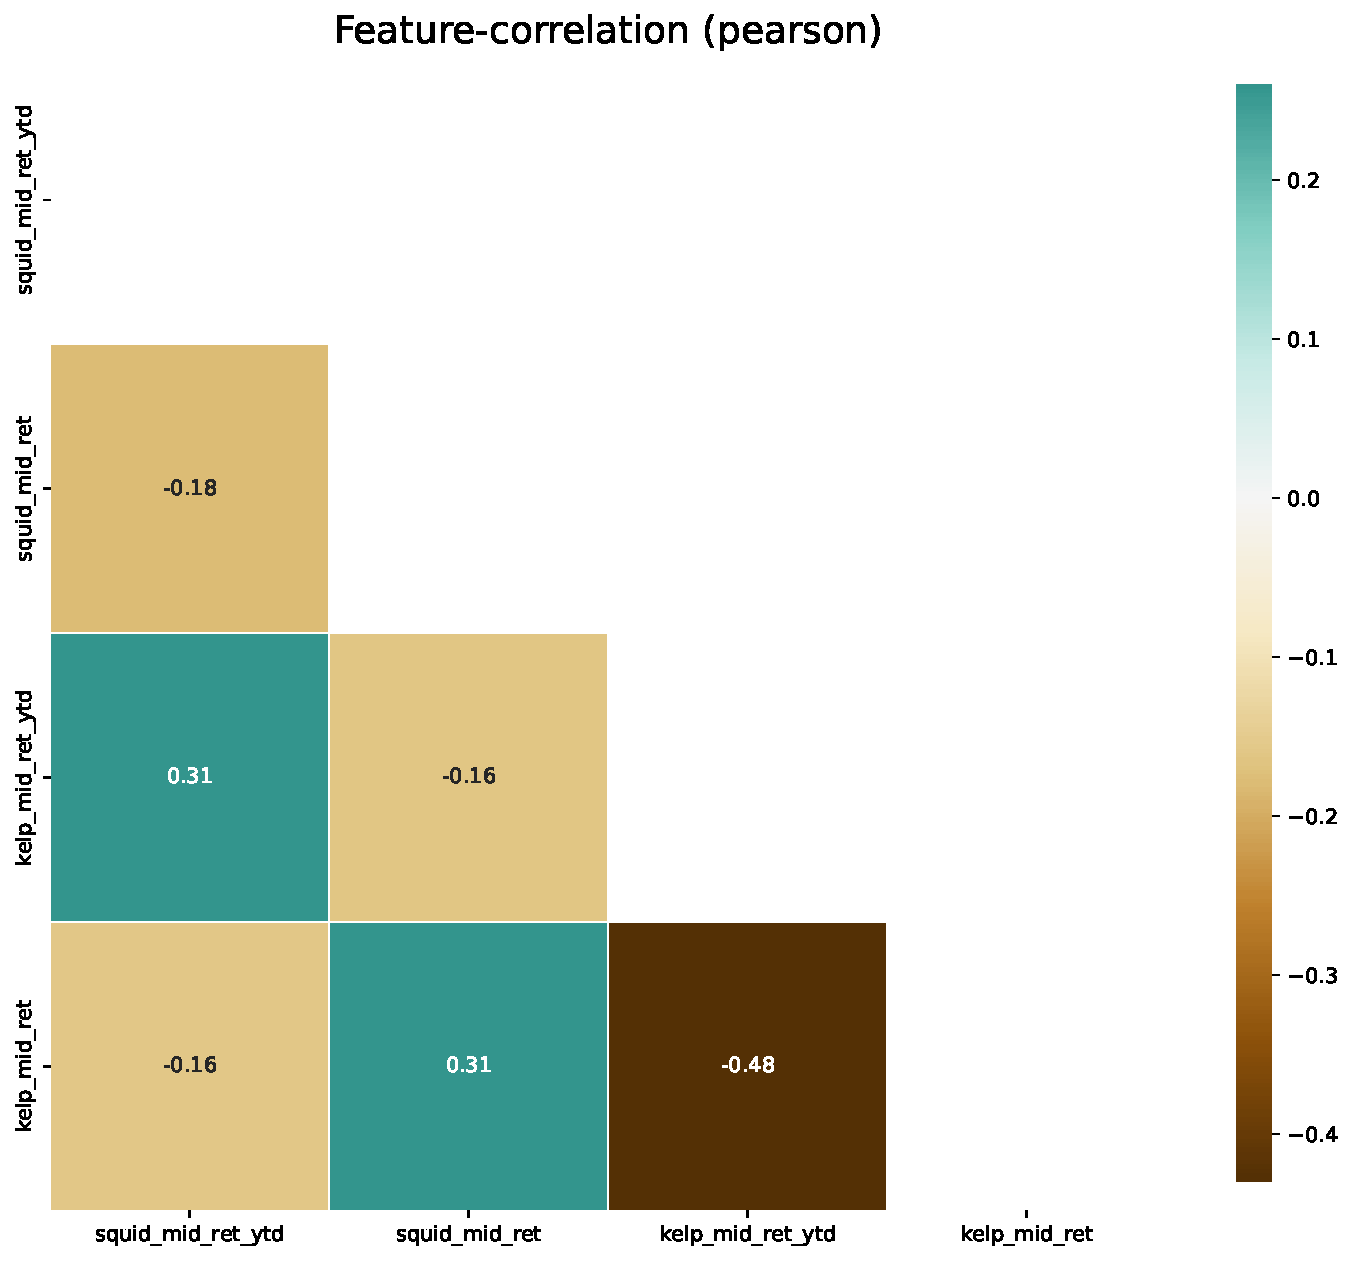
\includegraphics[keepaspectratio]{test_files/figure-pdf/cell-9-output-1.pdf}}

\begin{Shaded}
\begin{Highlighting}[]
\NormalTok{df\_m.set\_index([}\StringTok{\textquotesingle{}day\textquotesingle{}}\NormalTok{,}\StringTok{\textquotesingle{}timestamp\textquotesingle{}}\NormalTok{], inplace}\OperatorTok{=}\VariableTok{True}\NormalTok{)}
\end{Highlighting}
\end{Shaded}

\begin{Shaded}
\begin{Highlighting}[]
\ImportTok{import}\NormalTok{ pandas }\ImportTok{as}\NormalTok{ pd}
\ImportTok{import}\NormalTok{ numpy }\ImportTok{as}\NormalTok{ np}
\ImportTok{import}\NormalTok{ matplotlib.pyplot }\ImportTok{as}\NormalTok{ plt}
\ImportTok{import}\NormalTok{ seaborn }\ImportTok{as}\NormalTok{ sns}
\ImportTok{from}\NormalTok{ scipy }\ImportTok{import}\NormalTok{ stats}
\ImportTok{import}\NormalTok{ statsmodels.api }\ImportTok{as}\NormalTok{ sm}
\ImportTok{from}\NormalTok{ statsmodels.graphics.tsaplots }\ImportTok{import}\NormalTok{ plot\_acf, plot\_pacf}
\ImportTok{from}\NormalTok{ statsmodels.stats.diagnostic }\ImportTok{import}\NormalTok{ lilliefors}
\ImportTok{import}\NormalTok{ warnings}
\NormalTok{warnings.filterwarnings(}\StringTok{\textquotesingle{}ignore\textquotesingle{}}\NormalTok{)}
\end{Highlighting}
\end{Shaded}

\begin{Shaded}
\begin{Highlighting}[]
\CommentTok{\# Set the style for better visualizations}
\NormalTok{plt.style.use(}\StringTok{\textquotesingle{}seaborn{-}v0\_8{-}whitegrid\textquotesingle{}}\NormalTok{)}
\NormalTok{sns.set\_palette(}\StringTok{"deep"}\NormalTok{)}
\NormalTok{plt.rcParams[}\StringTok{\textquotesingle{}figure.figsize\textquotesingle{}}\NormalTok{] }\OperatorTok{=}\NormalTok{ [}\DecValTok{12}\NormalTok{, }\DecValTok{8}\NormalTok{]}
\end{Highlighting}
\end{Shaded}

\begin{Shaded}
\begin{Highlighting}[]
\ControlFlowTok{for}\NormalTok{ col }\KeywordTok{in}\NormalTok{ [}\StringTok{\textquotesingle{}squid\_mid\_ret\textquotesingle{}}\NormalTok{,}\StringTok{\textquotesingle{}kelp\_mid\_ret\textquotesingle{}}\NormalTok{]:}
    \CommentTok{\# Basic descriptive statistics}
\NormalTok{    stats\_df }\OperatorTok{=}\NormalTok{ pd.DataFrame(\{}
        \StringTok{\textquotesingle{}Statistic\textquotesingle{}}\NormalTok{: [}
            \StringTok{\textquotesingle{}Count\textquotesingle{}}\NormalTok{, }\StringTok{\textquotesingle{}Mean\textquotesingle{}}\NormalTok{, }\StringTok{\textquotesingle{}Median\textquotesingle{}}\NormalTok{, }\StringTok{\textquotesingle{}Std Dev\textquotesingle{}}\NormalTok{, }\StringTok{\textquotesingle{}Skewness\textquotesingle{}}\NormalTok{, }\StringTok{\textquotesingle{}Kurtosis\textquotesingle{}}\NormalTok{,}
            \StringTok{\textquotesingle{}Min\textquotesingle{}}\NormalTok{, }\StringTok{\textquotesingle{}Max\textquotesingle{}}\NormalTok{, }\StringTok{\textquotesingle{}25\%\textquotesingle{}}\NormalTok{, }\StringTok{\textquotesingle{}75\%\textquotesingle{}}\NormalTok{, }\StringTok{\textquotesingle{}Abs Mean\textquotesingle{}}\NormalTok{, }\StringTok{\textquotesingle{}Positive Returns \%\textquotesingle{}}
\NormalTok{        ],}
        \StringTok{\textquotesingle{}Value\textquotesingle{}}\NormalTok{: [}
\NormalTok{            df\_m[col].count(),}
\NormalTok{            df\_m[col].mean(),}
\NormalTok{            df\_m[col].median(),}
\NormalTok{            df\_m[col].std(),}
\NormalTok{            df\_m[col].skew(),}
\NormalTok{            df\_m[col].kurt(),}
\NormalTok{            df\_m[col].}\BuiltInTok{min}\NormalTok{(),}
\NormalTok{            df\_m[col].}\BuiltInTok{max}\NormalTok{(),}
\NormalTok{            df\_m[col].quantile(}\FloatTok{0.25}\NormalTok{),}
\NormalTok{            df\_m[col].quantile(}\FloatTok{0.75}\NormalTok{),}
\NormalTok{            df\_m[col].}\BuiltInTok{abs}\NormalTok{().mean(),}
\NormalTok{            (df\_m[col] }\OperatorTok{\textgreater{}} \DecValTok{0}\NormalTok{).mean() }\OperatorTok{*} \DecValTok{100}
\NormalTok{        ]}
\NormalTok{    \})}

    \BuiltInTok{print}\NormalTok{(stats\_df)}

    \CommentTok{\# Reset index to plot with timestamp}
\NormalTok{    df\_plot }\OperatorTok{=}\NormalTok{ df\_m.copy().reset\_index()}
\NormalTok{    df\_plot[}\StringTok{\textquotesingle{}index\textquotesingle{}}\NormalTok{] }\OperatorTok{=}\NormalTok{ ((df\_plot[}\StringTok{\textquotesingle{}day\textquotesingle{}}\NormalTok{]}\OperatorTok{+}\DecValTok{3}\NormalTok{)}\OperatorTok{*}\DecValTok{1000000}\NormalTok{) }\OperatorTok{+}\NormalTok{ df\_plot[}\StringTok{\textquotesingle{}timestamp\textquotesingle{}}\NormalTok{]}

    \CommentTok{\# Plotting the returns over time}
\NormalTok{    plt.figure(figsize}\OperatorTok{=}\NormalTok{(}\DecValTok{14}\NormalTok{, }\DecValTok{7}\NormalTok{))}
\NormalTok{    plt.plot(df\_plot[}\StringTok{\textquotesingle{}index\textquotesingle{}}\NormalTok{], df\_plot[col], linewidth}\OperatorTok{=}\FloatTok{1.5}\NormalTok{)}
\NormalTok{    plt.title(}\SpecialStringTok{f\textquotesingle{}}\SpecialCharTok{\{}\NormalTok{col}\SpecialCharTok{\}}\SpecialStringTok{ Returns Over Time\textquotesingle{}}\NormalTok{, fontsize}\OperatorTok{=}\DecValTok{16}\NormalTok{)}
\NormalTok{    plt.axhline(y}\OperatorTok{=}\DecValTok{0}\NormalTok{, color}\OperatorTok{=}\StringTok{\textquotesingle{}r\textquotesingle{}}\NormalTok{, linestyle}\OperatorTok{=}\StringTok{\textquotesingle{}{-}\textquotesingle{}}\NormalTok{, alpha}\OperatorTok{=}\FloatTok{0.3}\NormalTok{)}
\NormalTok{    plt.xlabel(}\StringTok{\textquotesingle{}Timestamp\textquotesingle{}}\NormalTok{)}
\NormalTok{    plt.ylabel(}\StringTok{\textquotesingle{}Returns\textquotesingle{}}\NormalTok{)}
\NormalTok{    plt.grid(}\VariableTok{True}\NormalTok{, alpha}\OperatorTok{=}\FloatTok{0.3}\NormalTok{)}
\NormalTok{    plt.show()}

    \CommentTok{\# Plot by day}

\NormalTok{    df\_plot2 }\OperatorTok{=}\NormalTok{ df\_plot.reset\_index()}

\NormalTok{    plt.figure(figsize}\OperatorTok{=}\NormalTok{(}\DecValTok{14}\NormalTok{, }\DecValTok{10}\NormalTok{))}
    \ControlFlowTok{for}\NormalTok{ day }\KeywordTok{in} \BuiltInTok{sorted}\NormalTok{(df\_plot2[}\StringTok{\textquotesingle{}day\textquotesingle{}}\NormalTok{].unique()):}
\NormalTok{        day\_data }\OperatorTok{=}\NormalTok{ df\_plot2[df\_plot2[}\StringTok{\textquotesingle{}day\textquotesingle{}}\NormalTok{] }\OperatorTok{==}\NormalTok{ day]}
\NormalTok{        plt.subplot(}\BuiltInTok{len}\NormalTok{(df\_plot2[}\StringTok{\textquotesingle{}day\textquotesingle{}}\NormalTok{].unique()), }\DecValTok{1}\NormalTok{, }\BuiltInTok{int}\NormalTok{(day) }\OperatorTok{+} \DecValTok{3}\NormalTok{)  }\CommentTok{\# +3 because days start at {-}2}
\NormalTok{        plt.plot(day\_data[}\StringTok{\textquotesingle{}timestamp\textquotesingle{}}\NormalTok{], day\_data[col], label}\OperatorTok{=}\SpecialStringTok{f\textquotesingle{}Day }\SpecialCharTok{\{}\NormalTok{day}\SpecialCharTok{\}}\SpecialStringTok{\textquotesingle{}}\NormalTok{)}
\NormalTok{        plt.axhline(y}\OperatorTok{=}\DecValTok{0}\NormalTok{, color}\OperatorTok{=}\StringTok{\textquotesingle{}r\textquotesingle{}}\NormalTok{, linestyle}\OperatorTok{=}\StringTok{\textquotesingle{}{-}\textquotesingle{}}\NormalTok{, alpha}\OperatorTok{=}\FloatTok{0.3}\NormalTok{)}
\NormalTok{        plt.title(}\SpecialStringTok{f\textquotesingle{}Day }\SpecialCharTok{\{}\NormalTok{day}\SpecialCharTok{\}}\SpecialStringTok{\textquotesingle{}}\NormalTok{)}
\NormalTok{        plt.grid(}\VariableTok{True}\NormalTok{, alpha}\OperatorTok{=}\FloatTok{0.3}\NormalTok{)}
\NormalTok{    plt.tight\_layout()}
\NormalTok{    plt.show()}

    \CommentTok{\# Histogram and KDE}
\NormalTok{    plt.figure(figsize}\OperatorTok{=}\NormalTok{(}\DecValTok{14}\NormalTok{, }\DecValTok{6}\NormalTok{))}

\NormalTok{    plt.subplot(}\DecValTok{1}\NormalTok{, }\DecValTok{2}\NormalTok{, }\DecValTok{1}\NormalTok{)}
\NormalTok{    sns.histplot(df\_m[col].dropna(), kde}\OperatorTok{=}\VariableTok{True}\NormalTok{, bins}\OperatorTok{=}\DecValTok{30}\NormalTok{)}
\NormalTok{    plt.axvline(x}\OperatorTok{=}\DecValTok{0}\NormalTok{, color}\OperatorTok{=}\StringTok{\textquotesingle{}r\textquotesingle{}}\NormalTok{, linestyle}\OperatorTok{=}\StringTok{\textquotesingle{}{-}{-}\textquotesingle{}}\NormalTok{, alpha}\OperatorTok{=}\FloatTok{0.7}\NormalTok{)}
\NormalTok{    plt.title(}\SpecialStringTok{f\textquotesingle{}Distribution of }\SpecialCharTok{\{}\NormalTok{col}\SpecialCharTok{\}}\SpecialStringTok{ Returns\textquotesingle{}}\NormalTok{, fontsize}\OperatorTok{=}\DecValTok{14}\NormalTok{)}
\NormalTok{    plt.xlabel(}\StringTok{\textquotesingle{}Returns\textquotesingle{}}\NormalTok{)}

\NormalTok{    plt.subplot(}\DecValTok{1}\NormalTok{, }\DecValTok{2}\NormalTok{, }\DecValTok{2}\NormalTok{)}
\NormalTok{    sns.boxplot(y}\OperatorTok{=}\NormalTok{df\_m[col].dropna())}
\NormalTok{    plt.title(}\SpecialStringTok{f\textquotesingle{}Box Plot of }\SpecialCharTok{\{}\NormalTok{col}\SpecialCharTok{\}}\SpecialStringTok{ Returns\textquotesingle{}}\NormalTok{, fontsize}\OperatorTok{=}\DecValTok{14}\NormalTok{)}
\NormalTok{    plt.ylabel(}\StringTok{\textquotesingle{}Returns\textquotesingle{}}\NormalTok{)}

\NormalTok{    plt.tight\_layout()}
\NormalTok{    plt.show()}

    \CommentTok{\# QQ Plot to check for normality}
\NormalTok{    plt.figure(figsize}\OperatorTok{=}\NormalTok{(}\DecValTok{10}\NormalTok{, }\DecValTok{6}\NormalTok{))}
\NormalTok{    sm.qqplot(df\_m[col].dropna(), line}\OperatorTok{=}\StringTok{\textquotesingle{}s\textquotesingle{}}\NormalTok{)}
\NormalTok{    plt.title(}\SpecialStringTok{f\textquotesingle{}QQ Plot of }\SpecialCharTok{\{}\NormalTok{col}\SpecialCharTok{\}}\SpecialStringTok{ Returns\textquotesingle{}}\NormalTok{, fontsize}\OperatorTok{=}\DecValTok{14}\NormalTok{)}
\NormalTok{    plt.grid(}\VariableTok{True}\NormalTok{, alpha}\OperatorTok{=}\FloatTok{0.3}\NormalTok{)}
\NormalTok{    plt.show()}

    \CommentTok{\# Run normality tests}
\NormalTok{    shapiro\_test }\OperatorTok{=}\NormalTok{ stats.shapiro(df\_m[col].dropna())}
\NormalTok{    ks\_test }\OperatorTok{=}\NormalTok{ lilliefors(df\_m[col].dropna())}
\NormalTok{    ad\_test }\OperatorTok{=}\NormalTok{ stats.anderson(df\_m[col].dropna(), dist}\OperatorTok{=}\StringTok{\textquotesingle{}norm\textquotesingle{}}\NormalTok{)}

    \BuiltInTok{print}\NormalTok{(}\SpecialStringTok{f"Normality Tests for }\SpecialCharTok{\{}\NormalTok{col}\SpecialCharTok{\}}\SpecialStringTok{ Returns:"}\NormalTok{)}
    \BuiltInTok{print}\NormalTok{(}\SpecialStringTok{f"Shapiro{-}Wilk Test: statistic=}\SpecialCharTok{\{}\NormalTok{shapiro\_test[}\DecValTok{0}\NormalTok{]}\SpecialCharTok{:.4f\}}\SpecialStringTok{, p{-}value=}\SpecialCharTok{\{}\NormalTok{shapiro\_test[}\DecValTok{1}\NormalTok{]}\SpecialCharTok{:.4f\}}\SpecialStringTok{"}\NormalTok{)}
    \BuiltInTok{print}\NormalTok{(}\SpecialStringTok{f"Kolmogorov{-}Smirnov Test: statistic=}\SpecialCharTok{\{}\NormalTok{ks\_test[}\DecValTok{0}\NormalTok{]}\SpecialCharTok{:.4f\}}\SpecialStringTok{, p{-}value=}\SpecialCharTok{\{}\NormalTok{ks\_test[}\DecValTok{1}\NormalTok{]}\SpecialCharTok{:.4f\}}\SpecialStringTok{"}\NormalTok{)}
    \BuiltInTok{print}\NormalTok{(}\StringTok{"Anderson{-}Darling Test:"}\NormalTok{)}
    \ControlFlowTok{for}\NormalTok{ i }\KeywordTok{in} \BuiltInTok{range}\NormalTok{(}\BuiltInTok{len}\NormalTok{(ad\_test.critical\_values)):}
\NormalTok{        sl, cv }\OperatorTok{=}\NormalTok{ ad\_test.significance\_level[i], ad\_test.critical\_values[i]}
        \BuiltInTok{print}\NormalTok{(}\SpecialStringTok{f"    }\SpecialCharTok{\{}\NormalTok{sl}\SpecialCharTok{\}}\SpecialStringTok{\%: }\SpecialCharTok{\{}\NormalTok{cv}\SpecialCharTok{:.3f\}}\SpecialStringTok{, }\SpecialCharTok{\{}\StringTok{\textquotesingle{}Reject\textquotesingle{}} \ControlFlowTok{if}\NormalTok{ ad\_test}\SpecialCharTok{.}\NormalTok{statistic }\OperatorTok{\textgreater{}}\NormalTok{ cv }\ControlFlowTok{else} \StringTok{\textquotesingle{}Accept\textquotesingle{}}\SpecialCharTok{\}}\SpecialStringTok{ null hypothesis"}\NormalTok{)}
    
    \CommentTok{\# Autocorrelation analysis}
\NormalTok{    fig, (ax1, ax2) }\OperatorTok{=}\NormalTok{ plt.subplots(}\DecValTok{1}\NormalTok{, }\DecValTok{2}\NormalTok{, figsize}\OperatorTok{=}\NormalTok{(}\DecValTok{14}\NormalTok{, }\DecValTok{5}\NormalTok{))}
\NormalTok{    plot\_acf(df\_m[col].dropna(), lags}\OperatorTok{=}\DecValTok{20}\NormalTok{, ax}\OperatorTok{=}\NormalTok{ax1)}
\NormalTok{    ax1.set\_title(}\StringTok{\textquotesingle{}Autocorrelation Function (ACF)\textquotesingle{}}\NormalTok{, fontsize}\OperatorTok{=}\DecValTok{14}\NormalTok{)}

\NormalTok{    plot\_pacf(df\_m[col].dropna(), lags}\OperatorTok{=}\DecValTok{20}\NormalTok{, ax}\OperatorTok{=}\NormalTok{ax2)}
\NormalTok{    ax2.set\_title(}\StringTok{\textquotesingle{}Partial Autocorrelation Function (PACF)\textquotesingle{}}\NormalTok{, fontsize}\OperatorTok{=}\DecValTok{14}\NormalTok{)}

\NormalTok{    plt.tight\_layout()}
\NormalTok{    plt.show()}

    \CommentTok{\# Calculate rolling statistics}
\NormalTok{    window\_sizes }\OperatorTok{=}\NormalTok{ [}\DecValTok{5}\NormalTok{, }\DecValTok{10}\NormalTok{, }\DecValTok{20}\NormalTok{]}
\NormalTok{    df\_rolling }\OperatorTok{=}\NormalTok{ df\_m.reset\_index()}

\NormalTok{    plt.figure(figsize}\OperatorTok{=}\NormalTok{(}\DecValTok{14}\NormalTok{, }\DecValTok{10}\NormalTok{))}

    \CommentTok{\# Rolling mean}
\NormalTok{    plt.subplot(}\DecValTok{3}\NormalTok{, }\DecValTok{1}\NormalTok{, }\DecValTok{1}\NormalTok{)}
\NormalTok{    plt.plot(df\_rolling[}\StringTok{\textquotesingle{}timestamp\textquotesingle{}}\NormalTok{], df\_rolling[col], label}\OperatorTok{=}\StringTok{\textquotesingle{}Returns\textquotesingle{}}\NormalTok{, alpha}\OperatorTok{=}\FloatTok{0.5}\NormalTok{)}
    \ControlFlowTok{for}\NormalTok{ window }\KeywordTok{in}\NormalTok{ window\_sizes:}
\NormalTok{        plt.plot(df\_rolling[}\StringTok{\textquotesingle{}timestamp\textquotesingle{}}\NormalTok{], }
\NormalTok{                df\_rolling[col].rolling(window}\OperatorTok{=}\NormalTok{window).mean(), }
\NormalTok{                label}\OperatorTok{=}\SpecialStringTok{f\textquotesingle{}}\SpecialCharTok{\{}\NormalTok{window}\SpecialCharTok{\}}\SpecialStringTok{{-}period MA\textquotesingle{}}\NormalTok{)}
\NormalTok{    plt.title(}\StringTok{\textquotesingle{}Rolling Mean of SQUID\_INK Returns\textquotesingle{}}\NormalTok{, fontsize}\OperatorTok{=}\DecValTok{14}\NormalTok{)}
\NormalTok{    plt.legend()}
\NormalTok{    plt.grid(}\VariableTok{True}\NormalTok{, alpha}\OperatorTok{=}\FloatTok{0.3}\NormalTok{)}

    \CommentTok{\# Rolling volatility (standard deviation)}
\NormalTok{    plt.subplot(}\DecValTok{3}\NormalTok{, }\DecValTok{1}\NormalTok{, }\DecValTok{2}\NormalTok{)}
    \ControlFlowTok{for}\NormalTok{ window }\KeywordTok{in}\NormalTok{ window\_sizes:}
\NormalTok{        plt.plot(df\_rolling[}\StringTok{\textquotesingle{}timestamp\textquotesingle{}}\NormalTok{], }
\NormalTok{                df\_rolling[col].rolling(window}\OperatorTok{=}\NormalTok{window).std(), }
\NormalTok{                label}\OperatorTok{=}\SpecialStringTok{f\textquotesingle{}}\SpecialCharTok{\{}\NormalTok{window}\SpecialCharTok{\}}\SpecialStringTok{{-}period SD\textquotesingle{}}\NormalTok{)}
\NormalTok{    plt.title(}\StringTok{\textquotesingle{}Rolling Volatility of SQUID\_INK Returns\textquotesingle{}}\NormalTok{, fontsize}\OperatorTok{=}\DecValTok{14}\NormalTok{)}
\NormalTok{    plt.legend()}
\NormalTok{    plt.grid(}\VariableTok{True}\NormalTok{, alpha}\OperatorTok{=}\FloatTok{0.3}\NormalTok{)}

    \CommentTok{\# Rolling min/max}
\NormalTok{    plt.subplot(}\DecValTok{3}\NormalTok{, }\DecValTok{1}\NormalTok{, }\DecValTok{3}\NormalTok{)}
    \ControlFlowTok{for}\NormalTok{ window }\KeywordTok{in}\NormalTok{ window\_sizes:}
\NormalTok{        plt.plot(df\_rolling[}\StringTok{\textquotesingle{}timestamp\textquotesingle{}}\NormalTok{], }
\NormalTok{                df\_rolling[col].rolling(window}\OperatorTok{=}\NormalTok{window).}\BuiltInTok{min}\NormalTok{(), }
\NormalTok{                label}\OperatorTok{=}\SpecialStringTok{f\textquotesingle{}}\SpecialCharTok{\{}\NormalTok{window}\SpecialCharTok{\}}\SpecialStringTok{{-}period Min\textquotesingle{}}\NormalTok{, linestyle}\OperatorTok{=}\StringTok{\textquotesingle{}{-}{-}\textquotesingle{}}\NormalTok{)}
\NormalTok{        plt.plot(df\_rolling[}\StringTok{\textquotesingle{}timestamp\textquotesingle{}}\NormalTok{], }
\NormalTok{                df\_rolling[col].rolling(window}\OperatorTok{=}\NormalTok{window).}\BuiltInTok{max}\NormalTok{(), }
\NormalTok{                label}\OperatorTok{=}\SpecialStringTok{f\textquotesingle{}}\SpecialCharTok{\{}\NormalTok{window}\SpecialCharTok{\}}\SpecialStringTok{{-}period Max\textquotesingle{}}\NormalTok{, linestyle}\OperatorTok{=}\StringTok{\textquotesingle{}{-}.\textquotesingle{}}\NormalTok{)}
\NormalTok{    plt.title(}\StringTok{\textquotesingle{}Rolling Min/Max of SQUID\_INK Returns\textquotesingle{}}\NormalTok{, fontsize}\OperatorTok{=}\DecValTok{14}\NormalTok{)}
\NormalTok{    plt.legend()}
\NormalTok{    plt.grid(}\VariableTok{True}\NormalTok{, alpha}\OperatorTok{=}\FloatTok{0.3}\NormalTok{)}

\NormalTok{    plt.tight\_layout()}
\NormalTok{    plt.show()}

    \CommentTok{\# Volatility clustering {-} plot squared returns}
\NormalTok{    plt.figure(figsize}\OperatorTok{=}\NormalTok{(}\DecValTok{14}\NormalTok{, }\DecValTok{6}\NormalTok{))}
\NormalTok{    plt.plot(df\_rolling[}\StringTok{\textquotesingle{}timestamp\textquotesingle{}}\NormalTok{], df\_rolling[col]}\OperatorTok{**}\DecValTok{2}\NormalTok{)}
\NormalTok{    plt.title(}\StringTok{\textquotesingle{}Squared Returns (Volatility Clustering)\textquotesingle{}}\NormalTok{, fontsize}\OperatorTok{=}\DecValTok{14}\NormalTok{)}
\NormalTok{    plt.xlabel(}\StringTok{\textquotesingle{}Timestamp\textquotesingle{}}\NormalTok{)}
\NormalTok{    plt.ylabel(}\StringTok{\textquotesingle{}Squared Returns\textquotesingle{}}\NormalTok{)}
\NormalTok{    plt.grid(}\VariableTok{True}\NormalTok{, alpha}\OperatorTok{=}\FloatTok{0.3}\NormalTok{)}
\NormalTok{    plt.show()}

    \CommentTok{\# ACF of absolute returns to check volatility persistence}
\NormalTok{    fig, (ax1, ax2) }\OperatorTok{=}\NormalTok{ plt.subplots(}\DecValTok{1}\NormalTok{, }\DecValTok{2}\NormalTok{, figsize}\OperatorTok{=}\NormalTok{(}\DecValTok{14}\NormalTok{, }\DecValTok{5}\NormalTok{))}
\NormalTok{    plot\_acf(df\_m[col].dropna().}\BuiltInTok{abs}\NormalTok{(), lags}\OperatorTok{=}\DecValTok{20}\NormalTok{, ax}\OperatorTok{=}\NormalTok{ax1)}
\NormalTok{    ax1.set\_title(}\StringTok{\textquotesingle{}ACF of Absolute Returns\textquotesingle{}}\NormalTok{, fontsize}\OperatorTok{=}\DecValTok{14}\NormalTok{)}

\NormalTok{    plot\_acf(df\_m[col].dropna()}\OperatorTok{**}\DecValTok{2}\NormalTok{, lags}\OperatorTok{=}\DecValTok{20}\NormalTok{, ax}\OperatorTok{=}\NormalTok{ax2)}
\NormalTok{    ax2.set\_title(}\StringTok{\textquotesingle{}ACF of Squared Returns\textquotesingle{}}\NormalTok{, fontsize}\OperatorTok{=}\DecValTok{14}\NormalTok{)}

\NormalTok{    plt.tight\_layout()}
\NormalTok{    plt.show()}

    \CommentTok{\# Correlation with Kelp returns}
\NormalTok{    plt.figure(figsize}\OperatorTok{=}\NormalTok{(}\DecValTok{14}\NormalTok{, }\DecValTok{6}\NormalTok{))}
\NormalTok{    plt.scatter(df\_m[}\StringTok{\textquotesingle{}kelp\_mid\_ret\textquotesingle{}}\NormalTok{], df\_m[col], alpha}\OperatorTok{=}\FloatTok{0.6}\NormalTok{)}
\NormalTok{    plt.title(}\StringTok{\textquotesingle{}SQUID\_INK Returns vs KELP Returns\textquotesingle{}}\NormalTok{, fontsize}\OperatorTok{=}\DecValTok{14}\NormalTok{)}
\NormalTok{    plt.xlabel(}\StringTok{\textquotesingle{}KELP Returns\textquotesingle{}}\NormalTok{)}
\NormalTok{    plt.ylabel(}\StringTok{\textquotesingle{}SQUID\_INK Returns\textquotesingle{}}\NormalTok{)}
\NormalTok{    plt.axhline(y}\OperatorTok{=}\DecValTok{0}\NormalTok{, color}\OperatorTok{=}\StringTok{\textquotesingle{}r\textquotesingle{}}\NormalTok{, linestyle}\OperatorTok{=}\StringTok{\textquotesingle{}{-}{-}\textquotesingle{}}\NormalTok{, alpha}\OperatorTok{=}\FloatTok{0.3}\NormalTok{)}
\NormalTok{    plt.axvline(x}\OperatorTok{=}\DecValTok{0}\NormalTok{, color}\OperatorTok{=}\StringTok{\textquotesingle{}r\textquotesingle{}}\NormalTok{, linestyle}\OperatorTok{=}\StringTok{\textquotesingle{}{-}{-}\textquotesingle{}}\NormalTok{, alpha}\OperatorTok{=}\FloatTok{0.3}\NormalTok{)}
\NormalTok{    plt.grid(}\VariableTok{True}\NormalTok{, alpha}\OperatorTok{=}\FloatTok{0.3}\NormalTok{)}

    \CommentTok{\# Add correlation coefficient to the plot}
\NormalTok{    corr }\OperatorTok{=}\NormalTok{ df\_m[[col, }\StringTok{\textquotesingle{}kelp\_mid\_ret\textquotesingle{}}\NormalTok{]].corr().iloc[}\DecValTok{0}\NormalTok{, }\DecValTok{1}\NormalTok{]}
\NormalTok{    plt.annotate(}\SpecialStringTok{f\textquotesingle{}Correlation: }\SpecialCharTok{\{}\NormalTok{corr}\SpecialCharTok{:.4f\}}\SpecialStringTok{\textquotesingle{}}\NormalTok{, }
\NormalTok{                xy}\OperatorTok{=}\NormalTok{(}\FloatTok{0.05}\NormalTok{, }\FloatTok{0.95}\NormalTok{), xycoords}\OperatorTok{=}\StringTok{\textquotesingle{}axes fraction\textquotesingle{}}\NormalTok{, }
\NormalTok{                bbox}\OperatorTok{=}\BuiltInTok{dict}\NormalTok{(boxstyle}\OperatorTok{=}\StringTok{"round,pad=0.3"}\NormalTok{, fc}\OperatorTok{=}\StringTok{"white"}\NormalTok{, ec}\OperatorTok{=}\StringTok{"b"}\NormalTok{, lw}\OperatorTok{=}\DecValTok{1}\NormalTok{))}
\NormalTok{    plt.show()}

    \CommentTok{\# Correlation over time}
\NormalTok{    window }\OperatorTok{=} \DecValTok{10}
\NormalTok{    df\_rolling[}\StringTok{\textquotesingle{}rolling\_corr\textquotesingle{}}\NormalTok{] }\OperatorTok{=}\NormalTok{ df\_rolling[col].rolling(window).corr(df\_rolling[}\StringTok{\textquotesingle{}kelp\_mid\_ret\textquotesingle{}}\NormalTok{])}

\NormalTok{    plt.figure(figsize}\OperatorTok{=}\NormalTok{(}\DecValTok{14}\NormalTok{, }\DecValTok{6}\NormalTok{))}
\NormalTok{    plt.plot(df\_rolling[}\StringTok{\textquotesingle{}timestamp\textquotesingle{}}\NormalTok{], df\_rolling[}\StringTok{\textquotesingle{}rolling\_corr\textquotesingle{}}\NormalTok{])}
\NormalTok{    plt.title(}\SpecialStringTok{f\textquotesingle{}Rolling }\SpecialCharTok{\{}\NormalTok{window}\SpecialCharTok{\}}\SpecialStringTok{{-}period Correlation between SQUID\_INK and KELP Returns\textquotesingle{}}\NormalTok{, fontsize}\OperatorTok{=}\DecValTok{14}\NormalTok{)}
\NormalTok{    plt.xlabel(}\StringTok{\textquotesingle{}Timestamp\textquotesingle{}}\NormalTok{)}
\NormalTok{    plt.ylabel(}\StringTok{\textquotesingle{}Correlation\textquotesingle{}}\NormalTok{)}
\NormalTok{    plt.axhline(y}\OperatorTok{=}\DecValTok{0}\NormalTok{, color}\OperatorTok{=}\StringTok{\textquotesingle{}r\textquotesingle{}}\NormalTok{, linestyle}\OperatorTok{=}\StringTok{\textquotesingle{}{-}{-}\textquotesingle{}}\NormalTok{, alpha}\OperatorTok{=}\FloatTok{0.3}\NormalTok{)}
\NormalTok{    plt.grid(}\VariableTok{True}\NormalTok{, alpha}\OperatorTok{=}\FloatTok{0.3}\NormalTok{)}
\NormalTok{    plt.show()}

    \CommentTok{\# Compare return distributions by day}
\NormalTok{    plt.figure(figsize}\OperatorTok{=}\NormalTok{(}\DecValTok{14}\NormalTok{, }\DecValTok{6}\NormalTok{))}
\NormalTok{    sns.violinplot(x}\OperatorTok{=}\StringTok{\textquotesingle{}day\textquotesingle{}}\NormalTok{, y}\OperatorTok{=}\NormalTok{col, data}\OperatorTok{=}\NormalTok{df\_rolling)}
\NormalTok{    plt.title(}\StringTok{\textquotesingle{}Distribution of SQUID\_INK Returns by Day\textquotesingle{}}\NormalTok{, fontsize}\OperatorTok{=}\DecValTok{14}\NormalTok{)}
\NormalTok{    plt.xlabel(}\StringTok{\textquotesingle{}Day\textquotesingle{}}\NormalTok{)}
\NormalTok{    plt.ylabel(}\StringTok{\textquotesingle{}Returns\textquotesingle{}}\NormalTok{)}
\NormalTok{    plt.grid(}\VariableTok{True}\NormalTok{, alpha}\OperatorTok{=}\FloatTok{0.3}\NormalTok{)}
\NormalTok{    plt.show()}
\end{Highlighting}
\end{Shaded}

\begin{verbatim}
             Statistic         Value
0                Count  29999.000000
1                 Mean     -0.000002
2               Median      0.000000
3              Std Dev      0.000912
4             Skewness     -3.308303
5             Kurtosis    559.090015
6                  Min     -0.053963
7                  Max      0.039301
8                  25%     -0.000502
9                  75%      0.000503
10            Abs Mean      0.000563
11  Positive Returns %     40.783333
\end{verbatim}

\pandocbounded{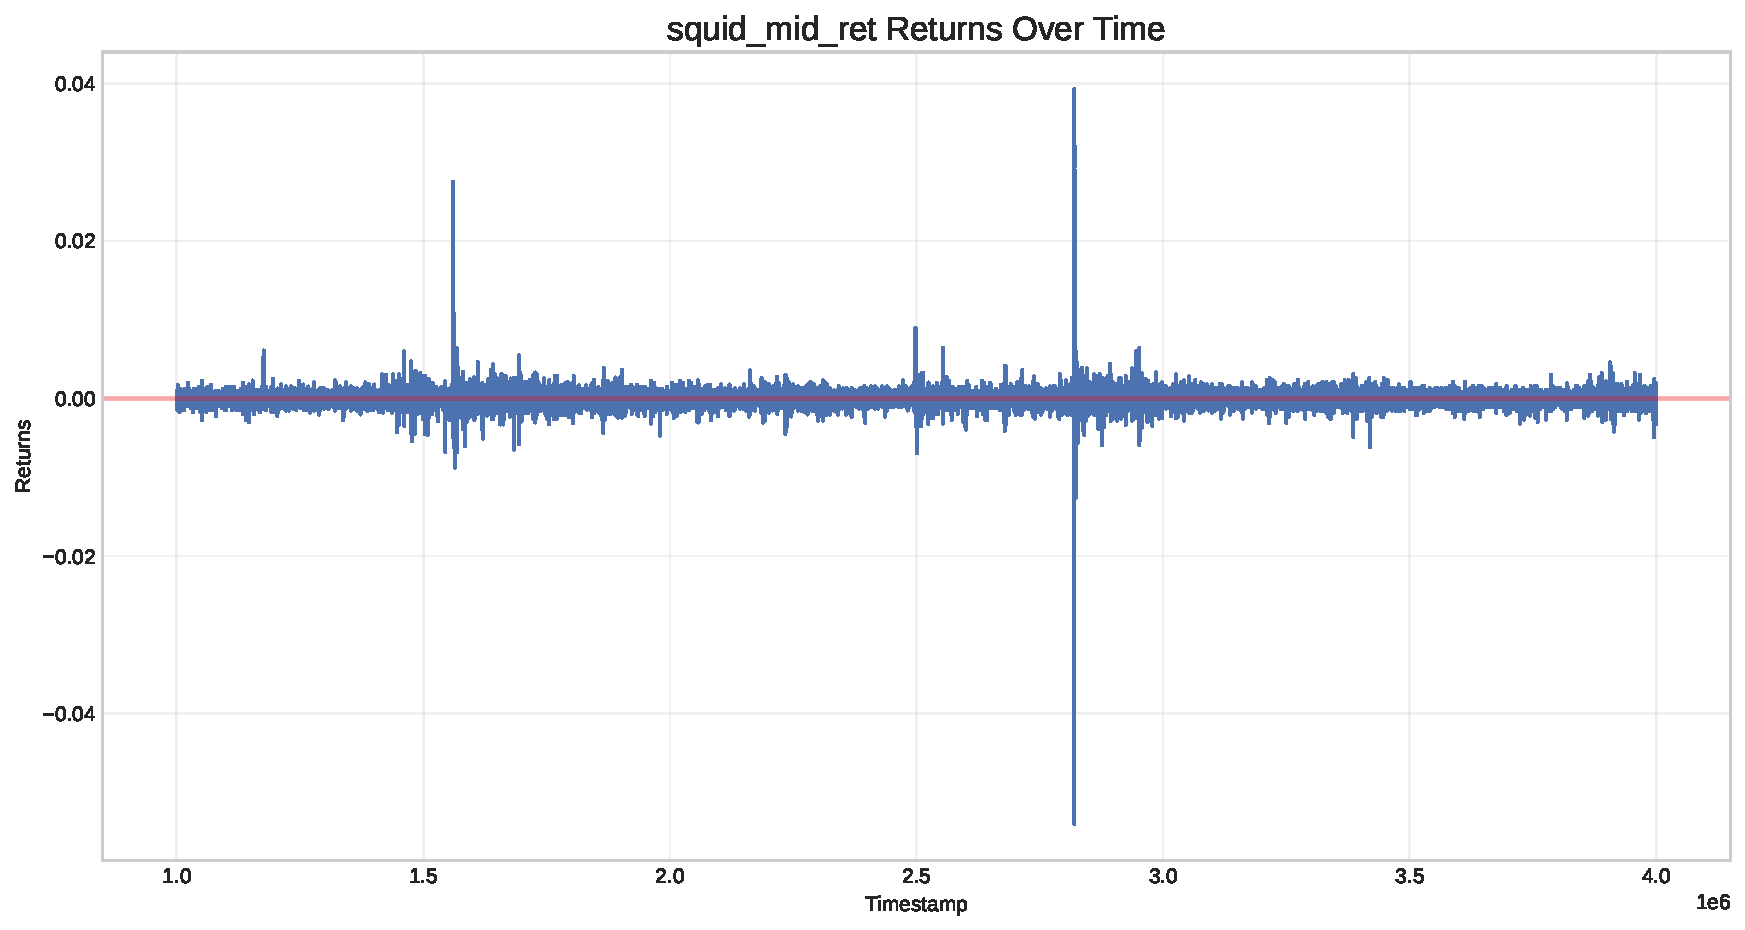
\includegraphics[keepaspectratio]{test_files/figure-pdf/cell-13-output-2.pdf}}

\pandocbounded{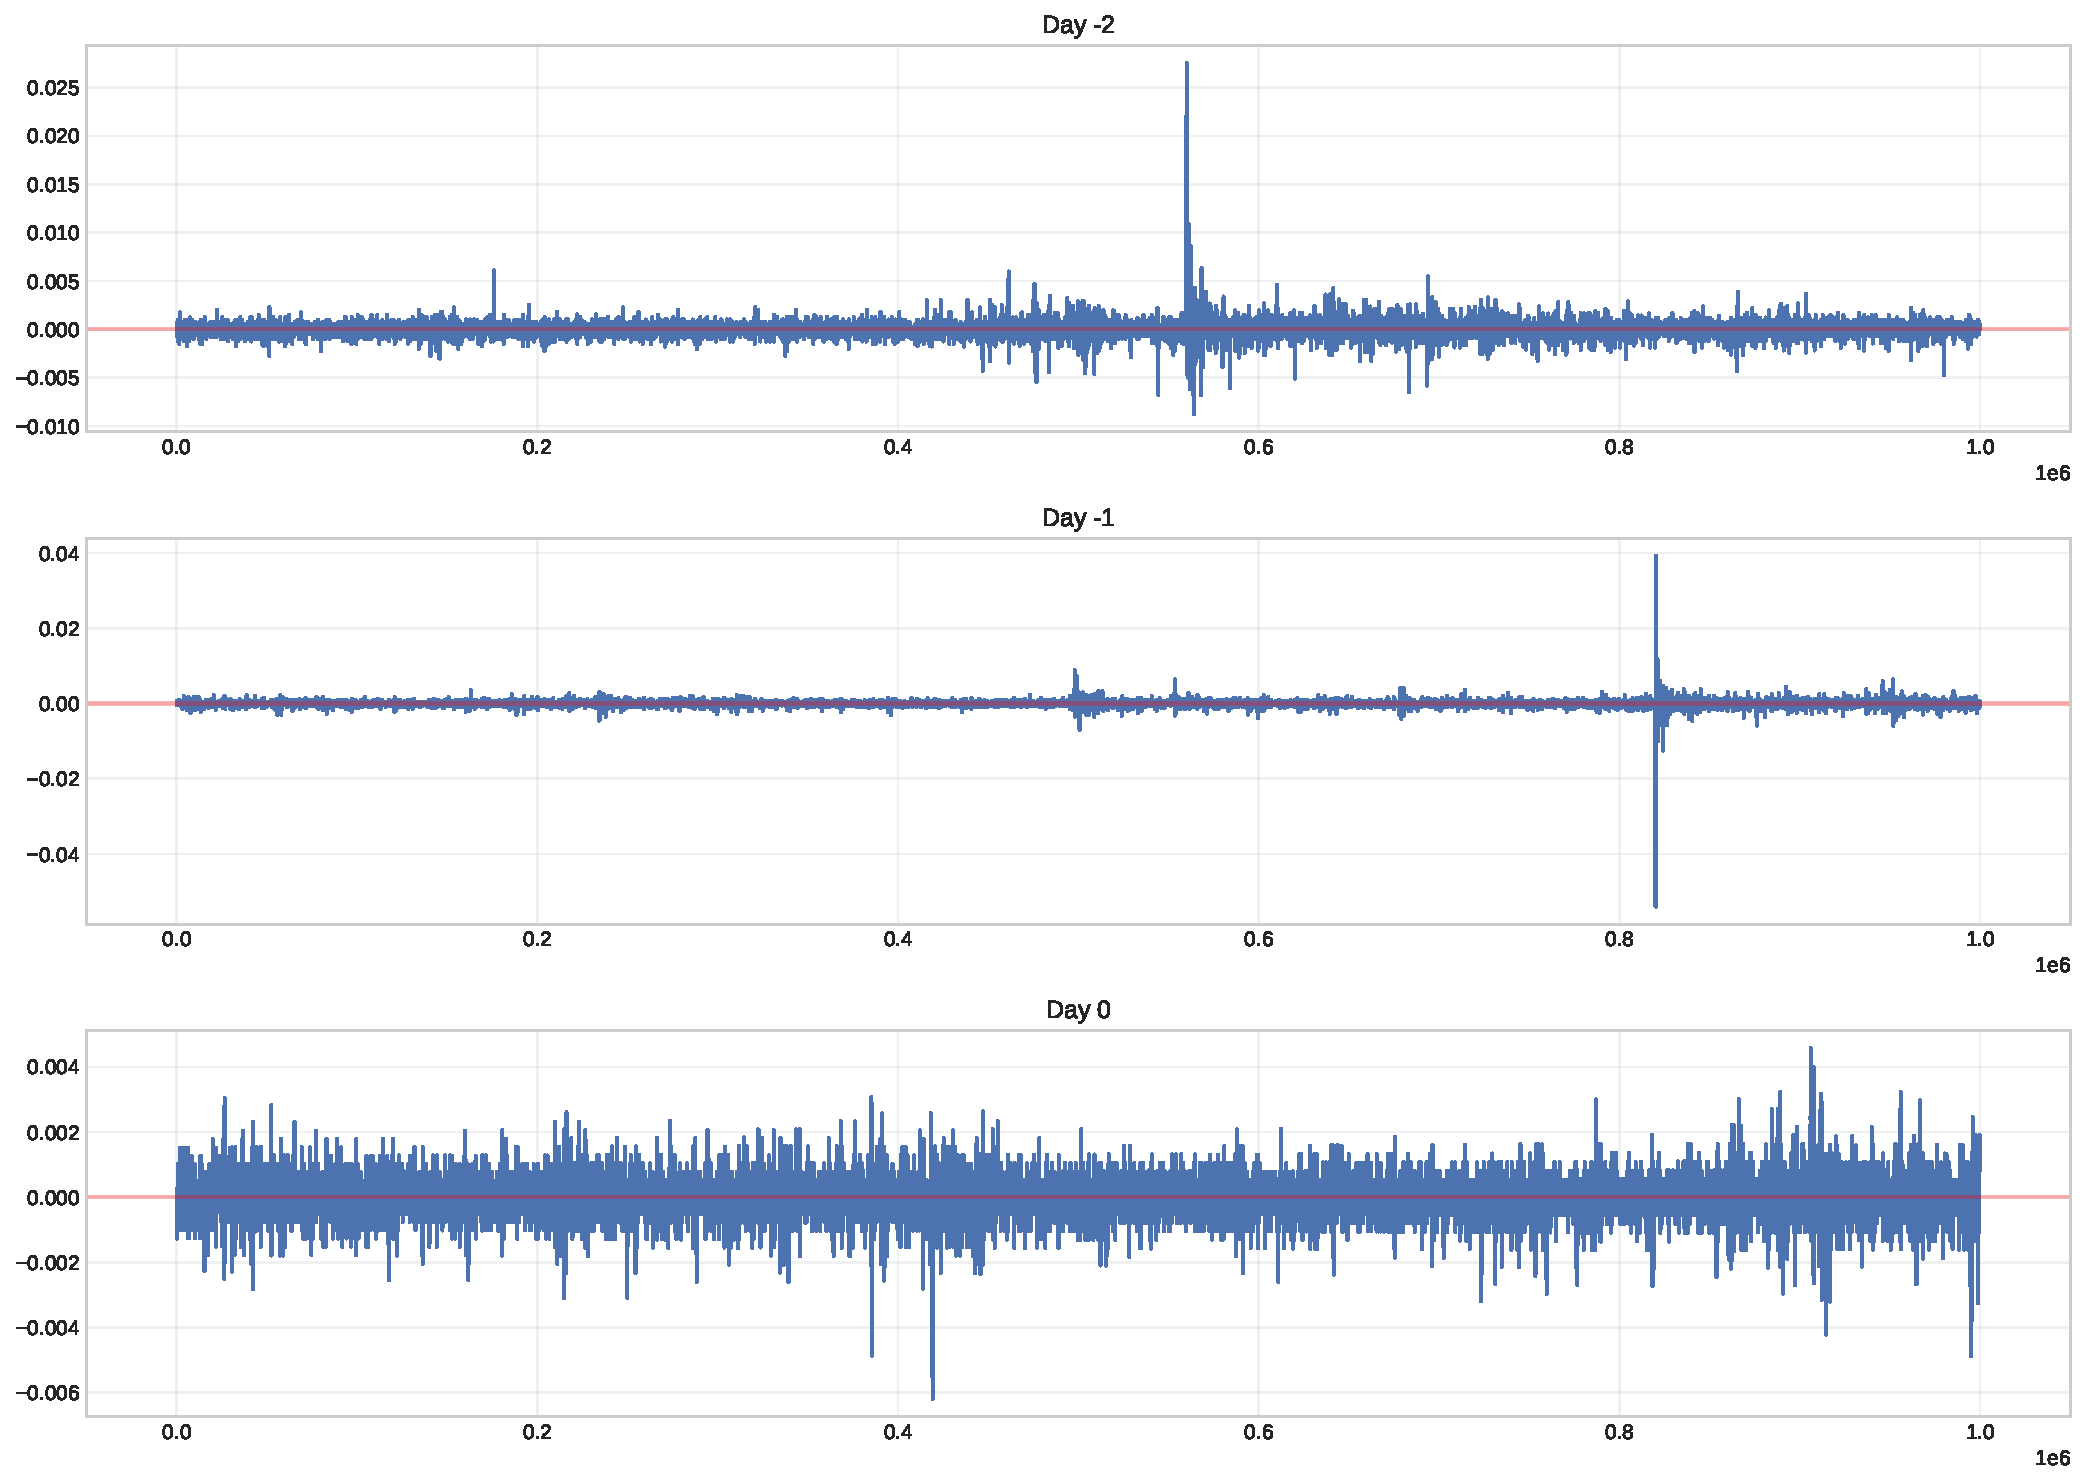
\includegraphics[keepaspectratio]{test_files/figure-pdf/cell-13-output-3.pdf}}

\pandocbounded{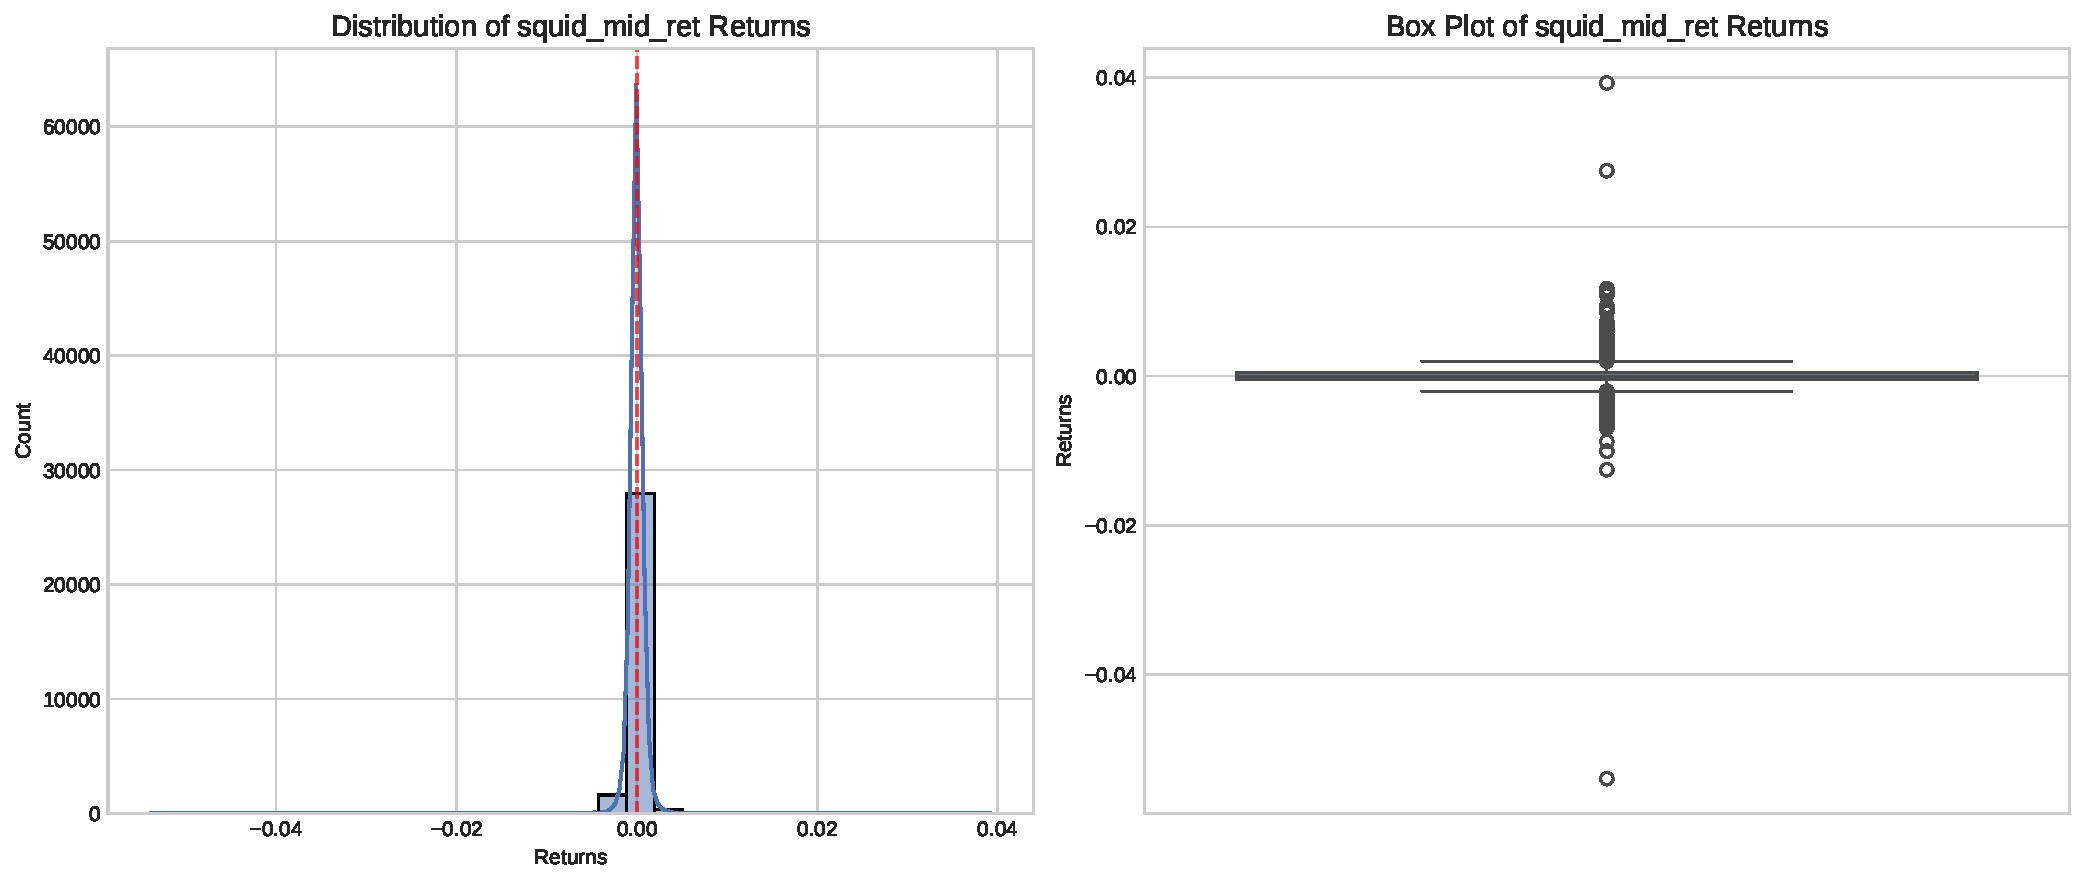
\includegraphics[keepaspectratio]{test_files/figure-pdf/cell-13-output-4.pdf}}

\begin{verbatim}
<Figure size 3000x1800 with 0 Axes>
\end{verbatim}

\pandocbounded{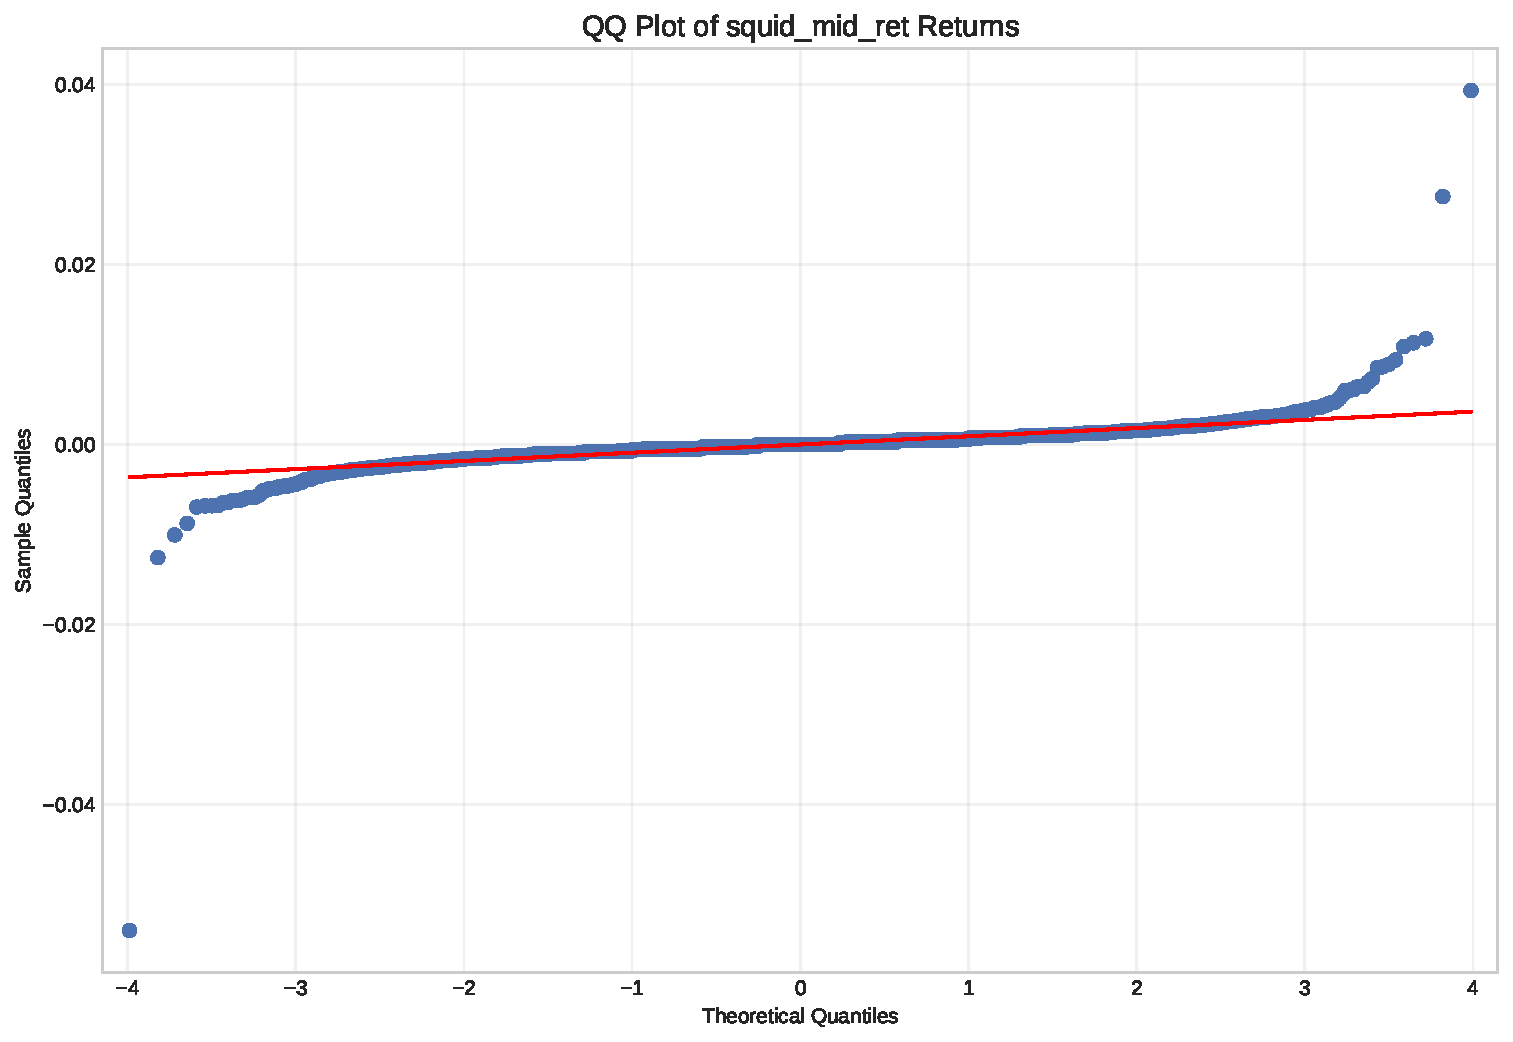
\includegraphics[keepaspectratio]{test_files/figure-pdf/cell-13-output-6.pdf}}

\begin{verbatim}
Normality Tests for squid_mid_ret Returns:
Shapiro-Wilk Test: statistic=0.7528, p-value=0.0000
Kolmogorov-Smirnov Test: statistic=0.1146, p-value=0.0010
Anderson-Darling Test:
    15.0%: 0.576, Reject null hypothesis
    10.0%: 0.656, Reject null hypothesis
    5.0%: 0.787, Reject null hypothesis
    2.5%: 0.918, Reject null hypothesis
    1.0%: 1.092, Reject null hypothesis
\end{verbatim}

\pandocbounded{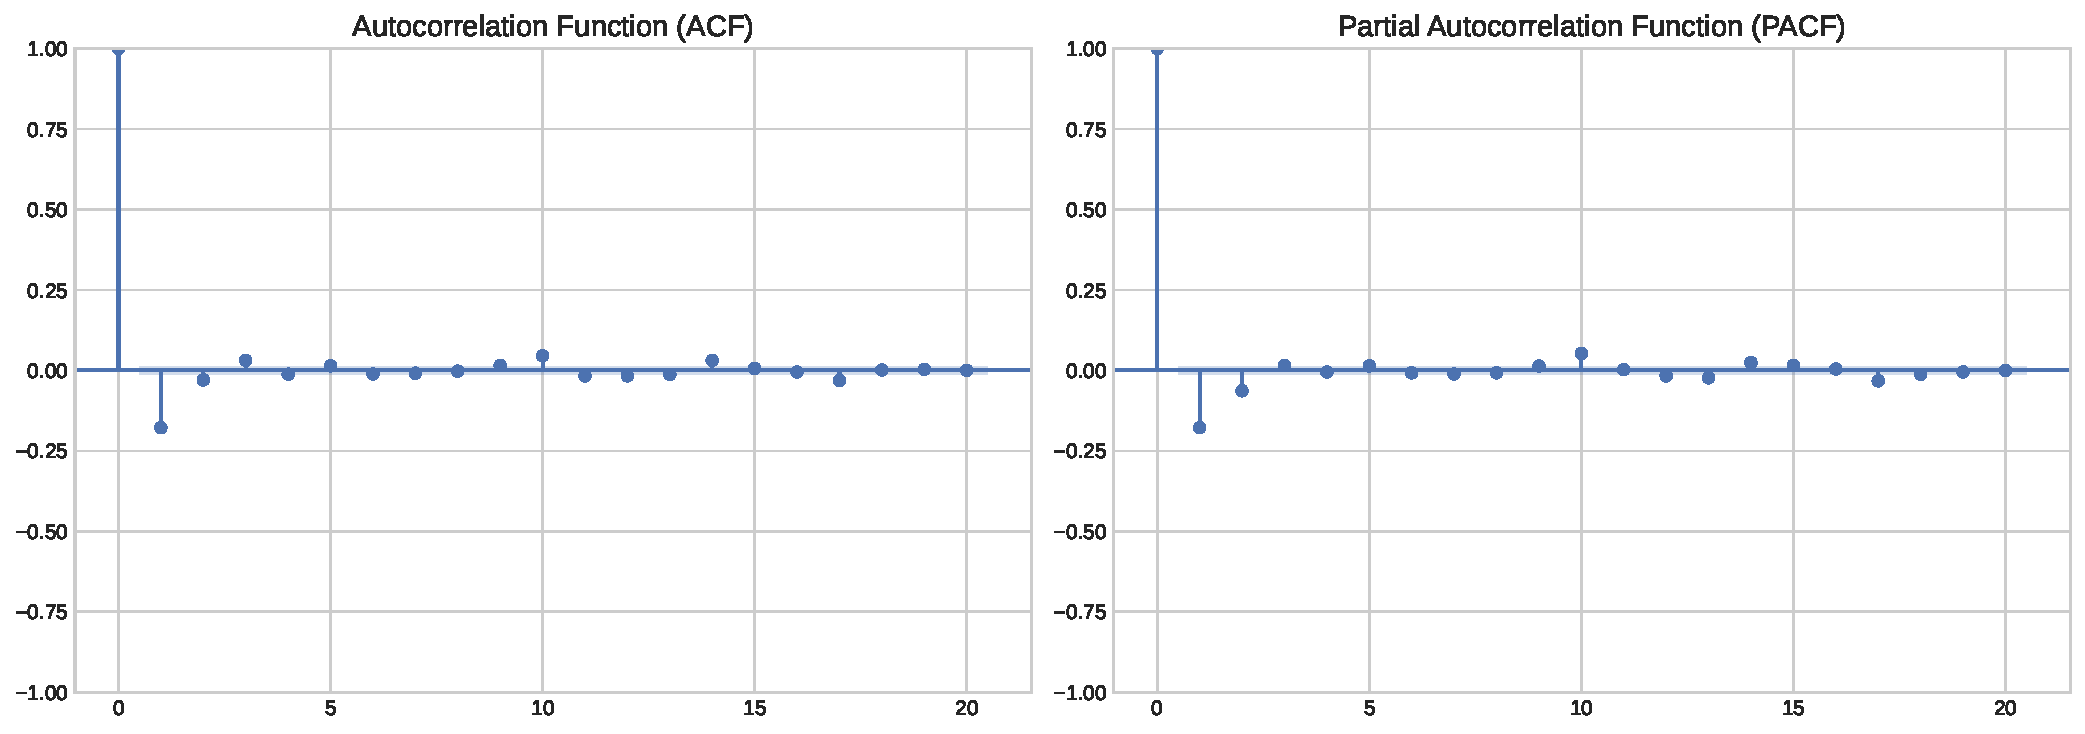
\includegraphics[keepaspectratio]{test_files/figure-pdf/cell-13-output-8.pdf}}

\pandocbounded{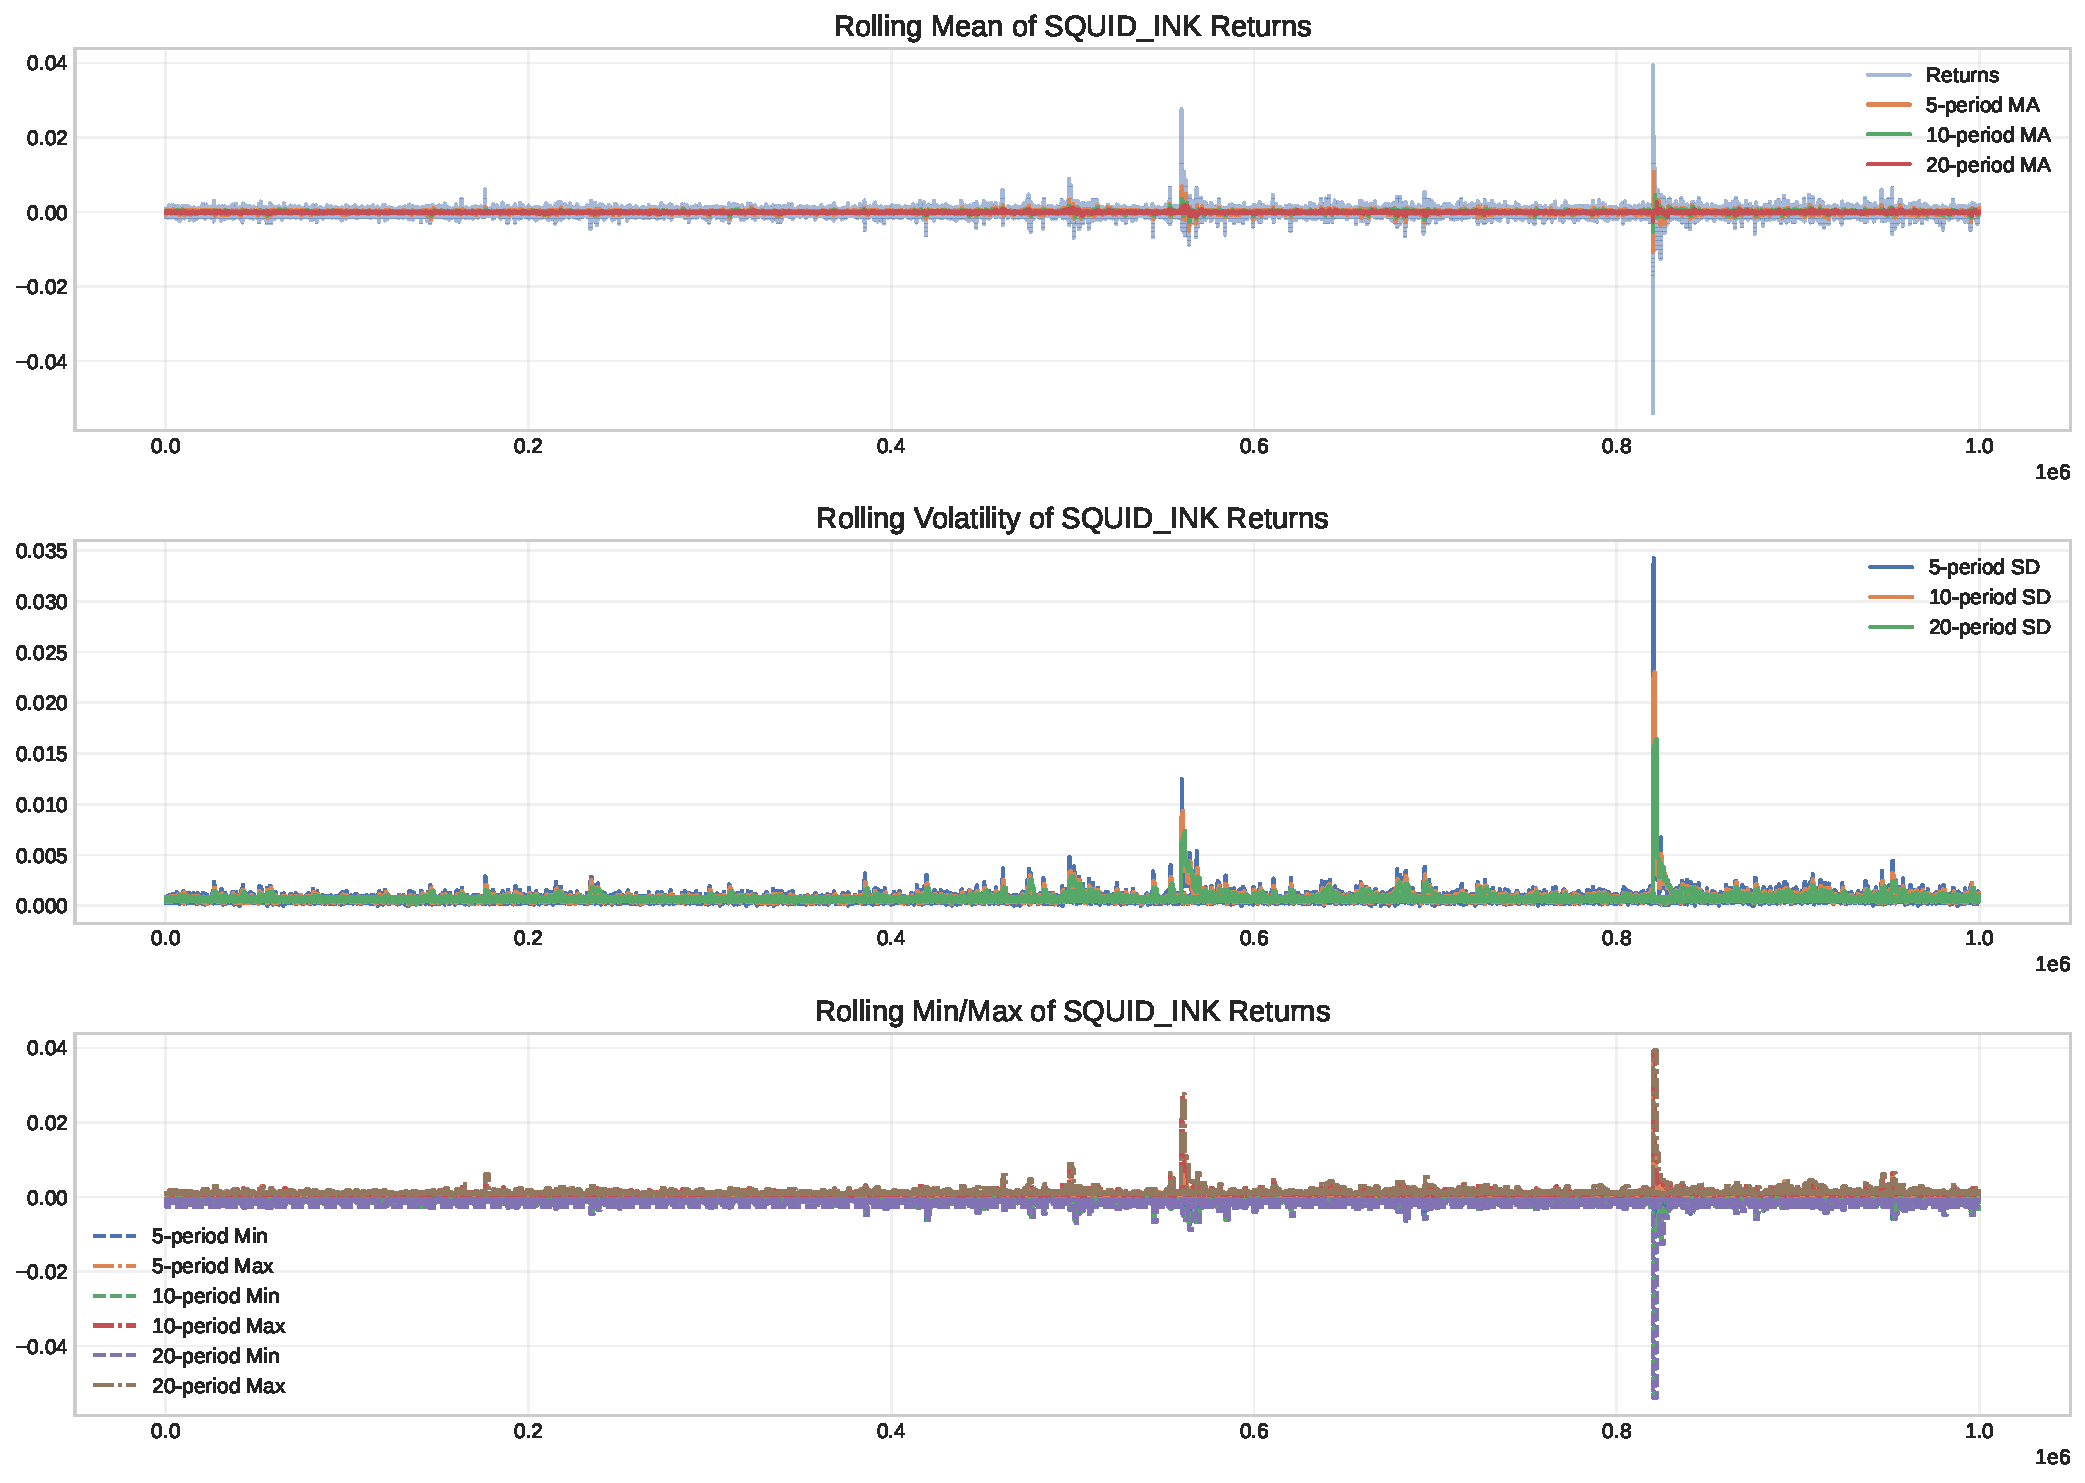
\includegraphics[keepaspectratio]{test_files/figure-pdf/cell-13-output-9.pdf}}

\pandocbounded{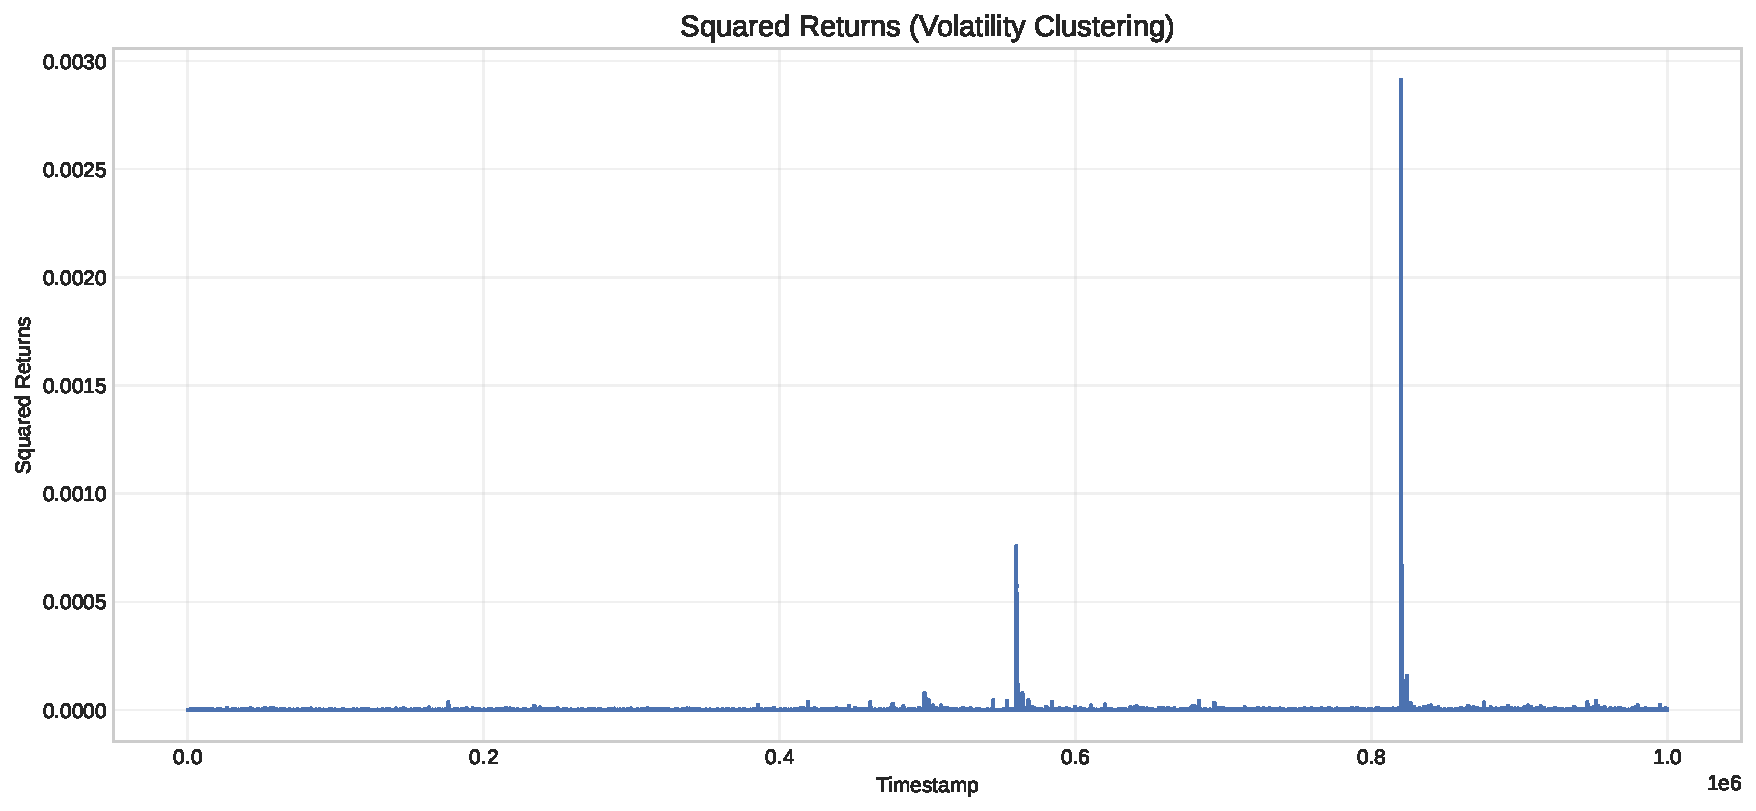
\includegraphics[keepaspectratio]{test_files/figure-pdf/cell-13-output-10.pdf}}

\pandocbounded{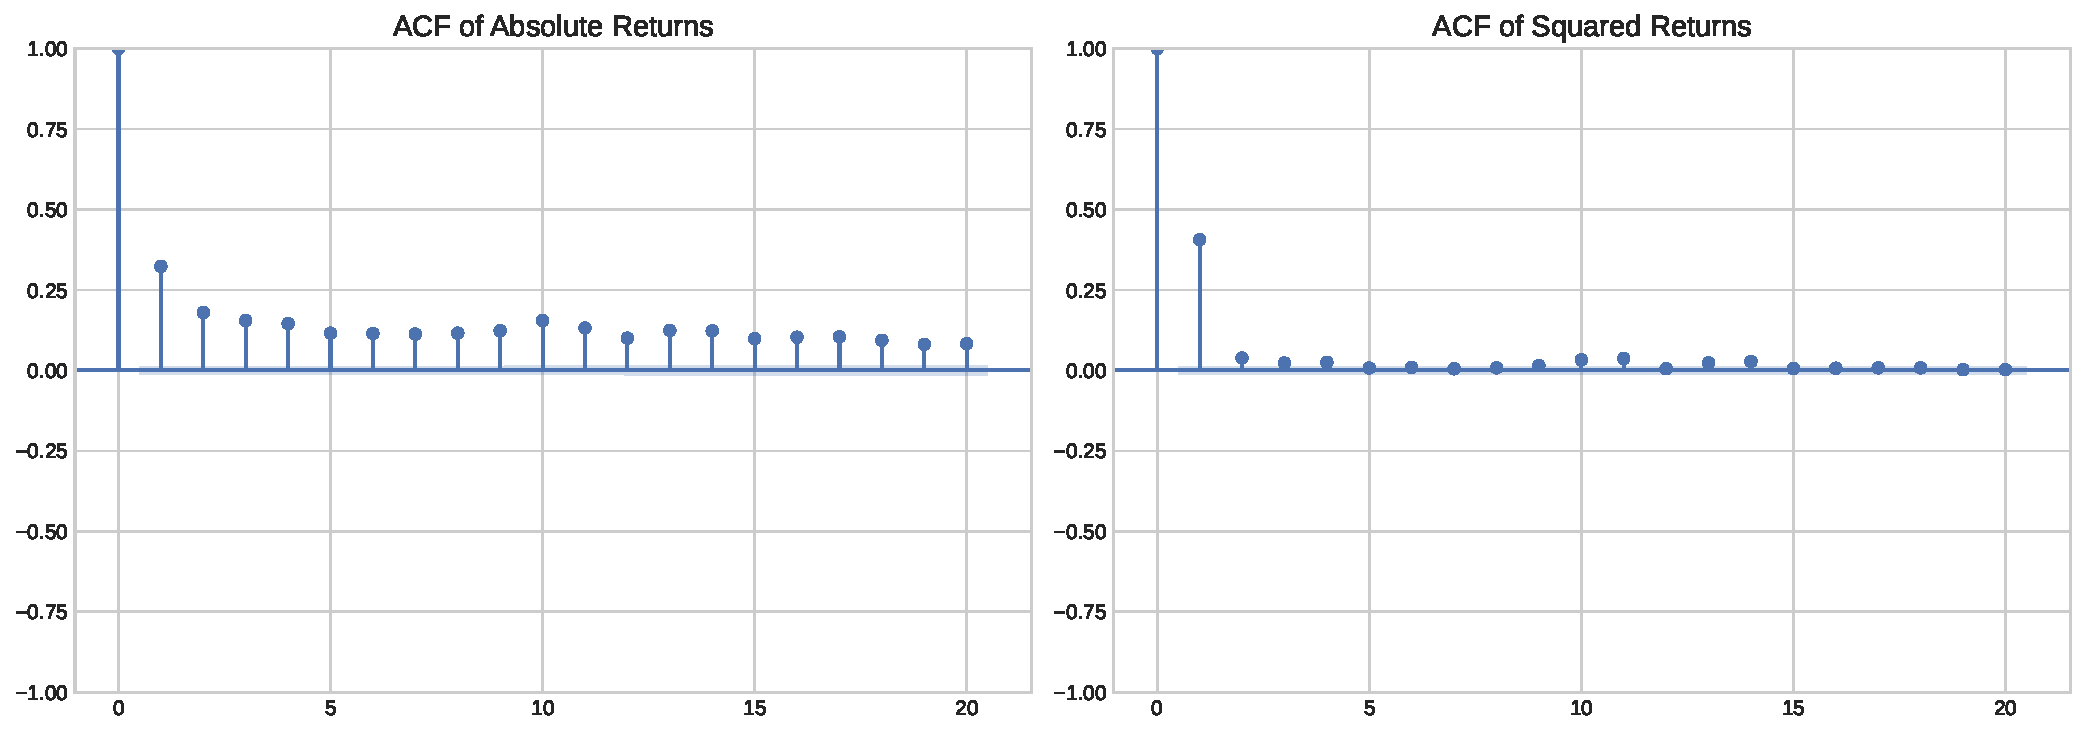
\includegraphics[keepaspectratio]{test_files/figure-pdf/cell-13-output-11.pdf}}

\pandocbounded{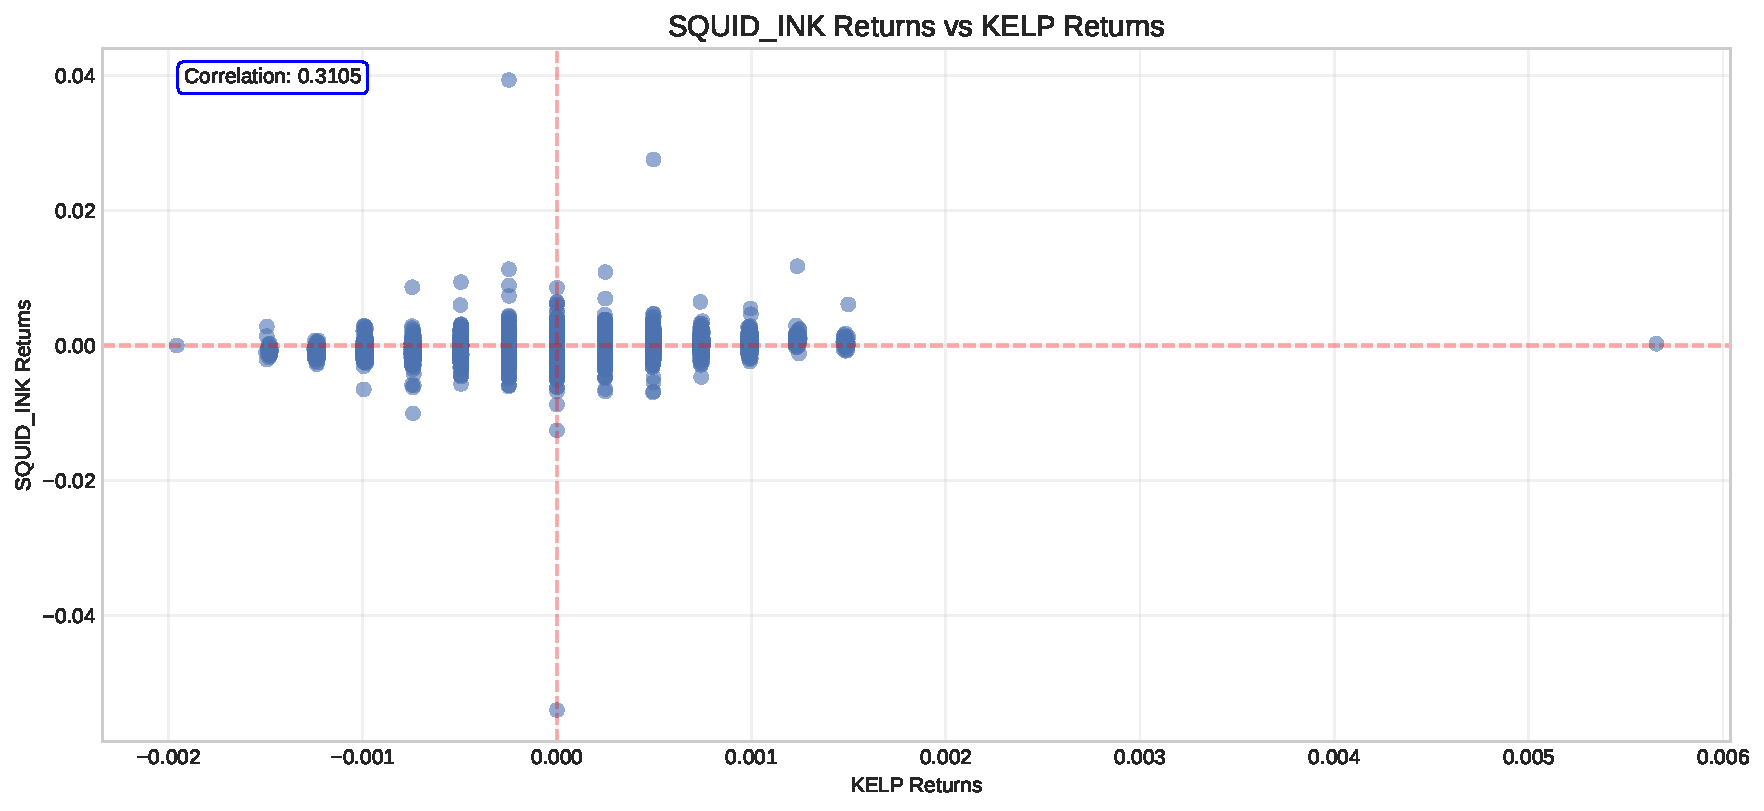
\includegraphics[keepaspectratio]{test_files/figure-pdf/cell-13-output-12.pdf}}

\pandocbounded{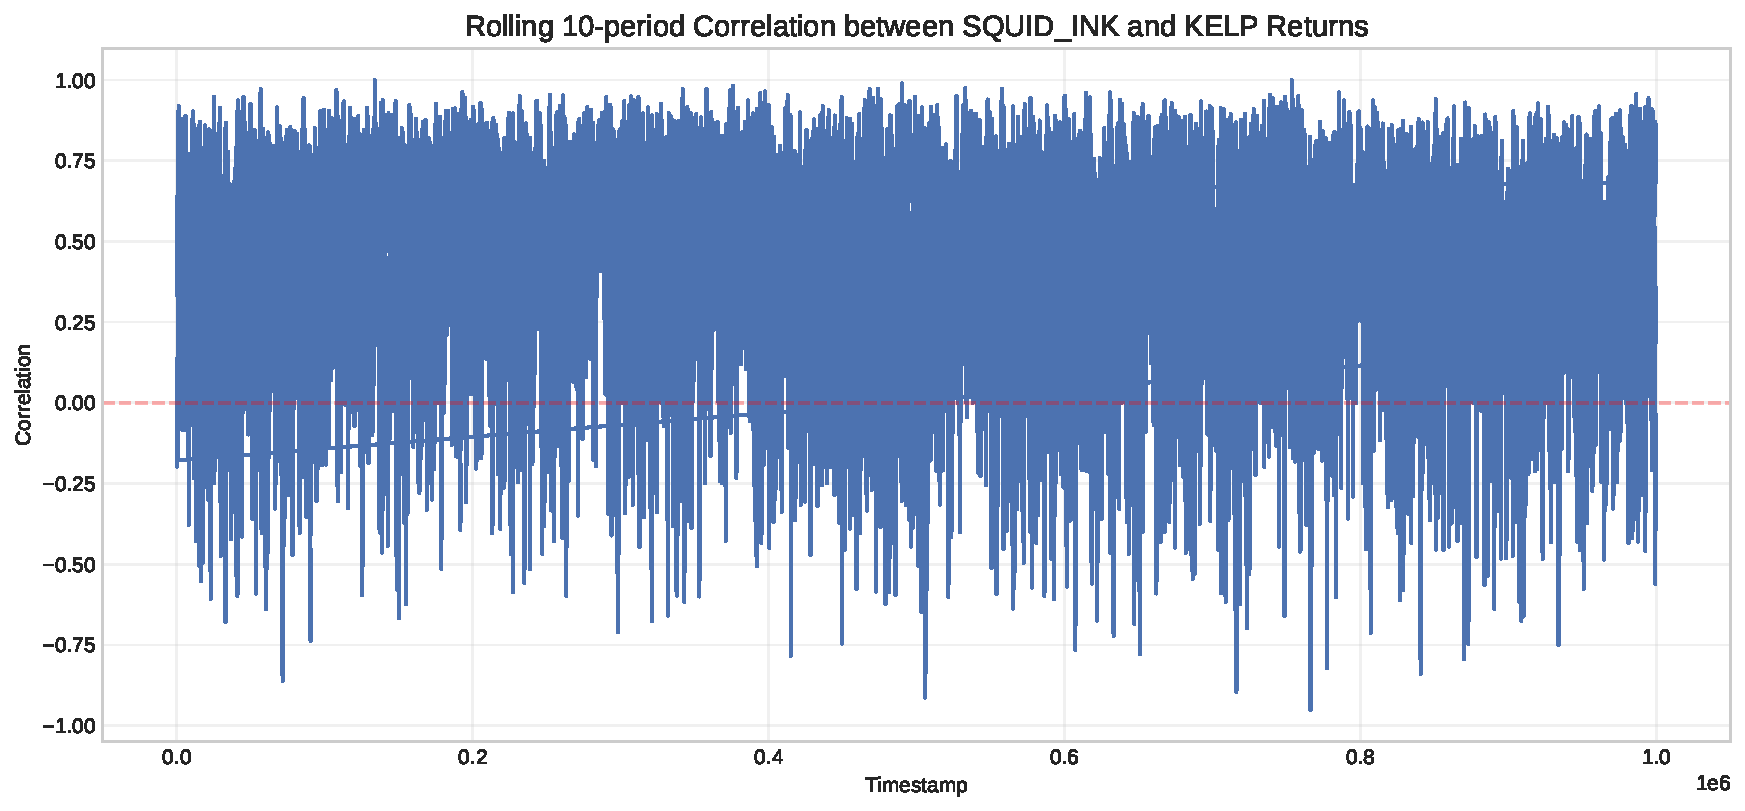
\includegraphics[keepaspectratio]{test_files/figure-pdf/cell-13-output-13.pdf}}

\pandocbounded{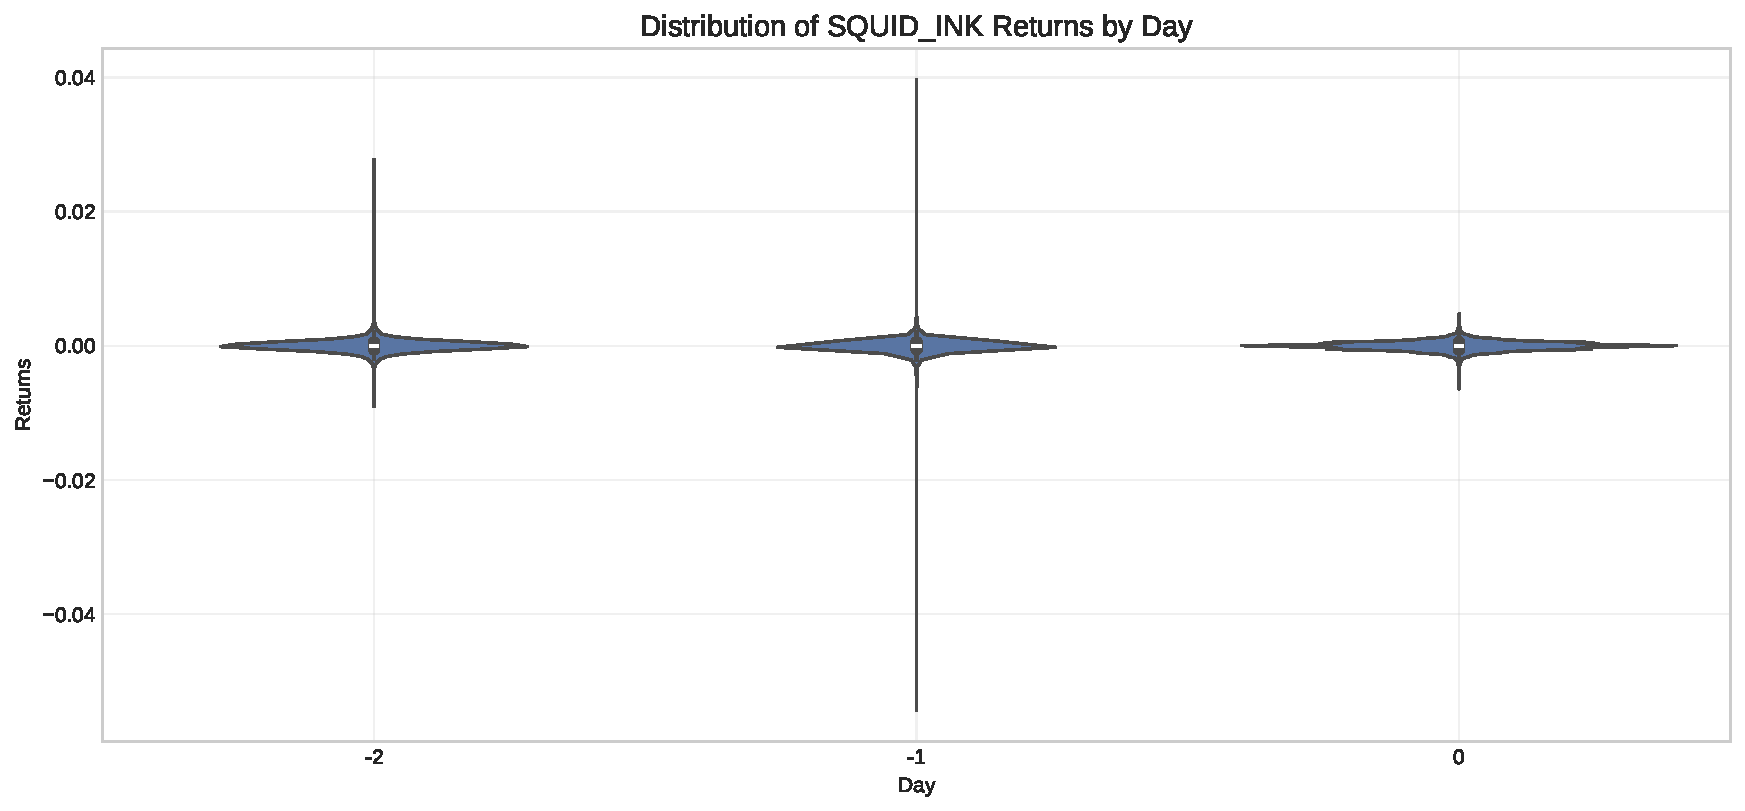
\includegraphics[keepaspectratio]{test_files/figure-pdf/cell-13-output-14.pdf}}

\begin{verbatim}
             Statistic         Value
0                Count  2.999900e+04
1                 Mean  6.283120e-07
2               Median  0.000000e+00
3              Std Dev  3.862354e-04
4             Skewness  9.796893e-02
5             Kurtosis  2.386128e+00
6                  Min -1.956469e-03
7                  Max  5.656665e-03
8                  25% -2.461841e-04
9                  75%  2.463054e-04
10            Abs Mean  2.650698e-04
11  Positive Returns %  3.049333e+01
\end{verbatim}

\pandocbounded{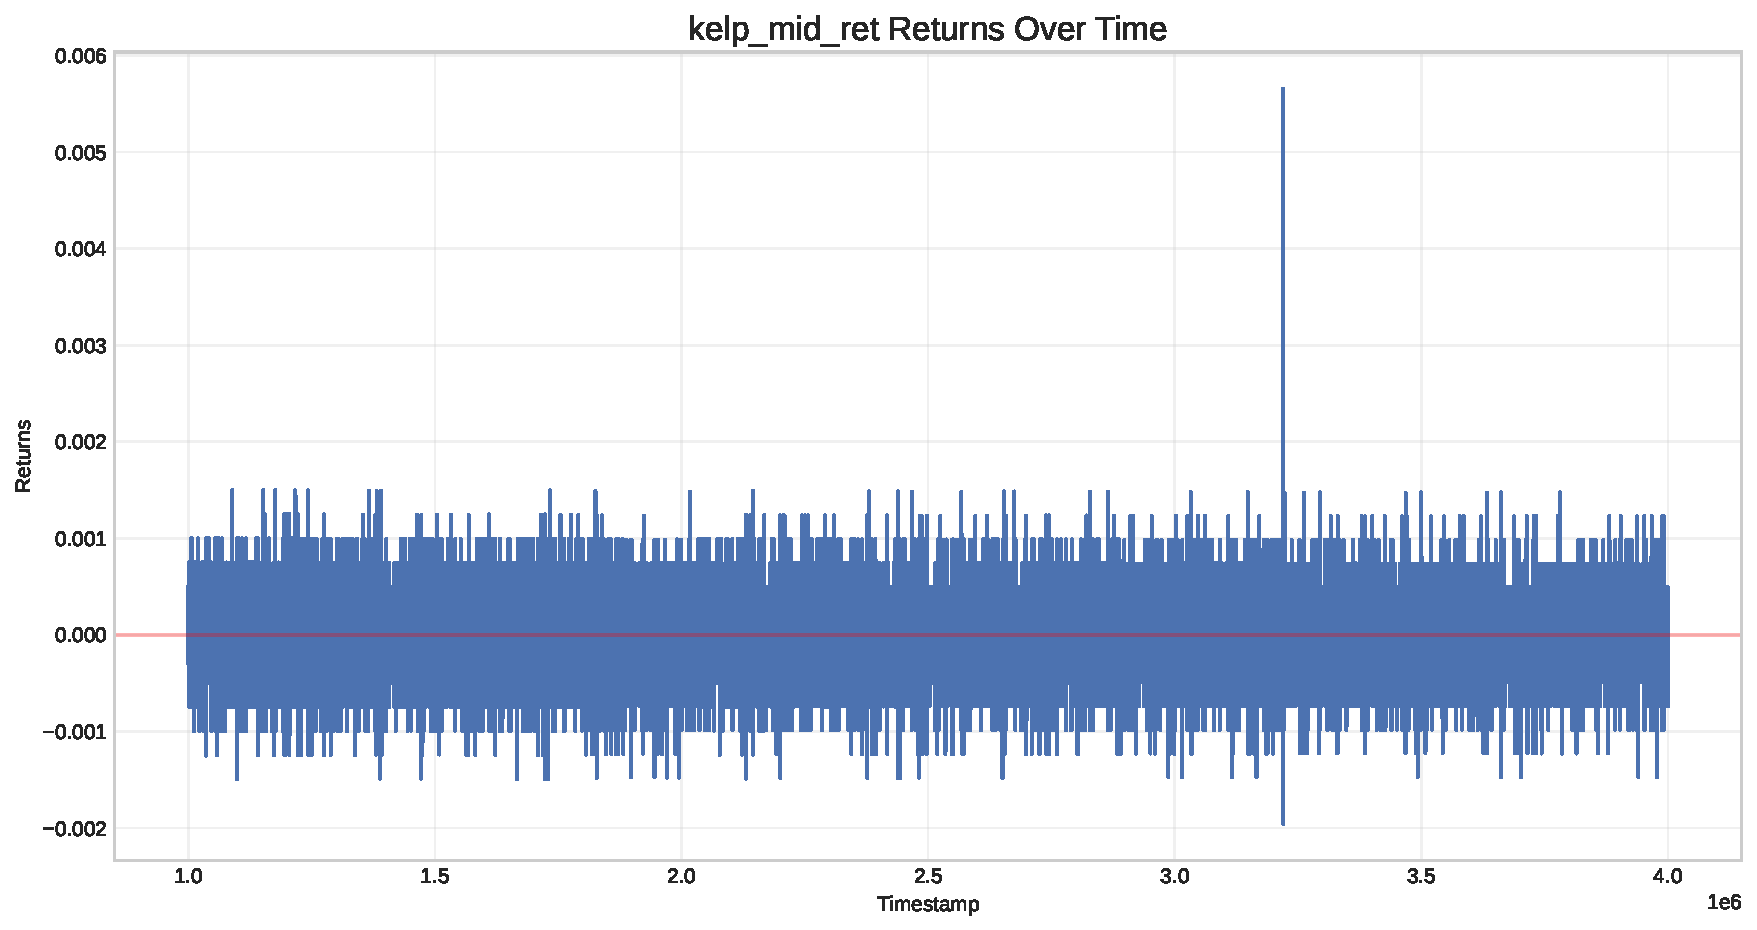
\includegraphics[keepaspectratio]{test_files/figure-pdf/cell-13-output-16.pdf}}

\pandocbounded{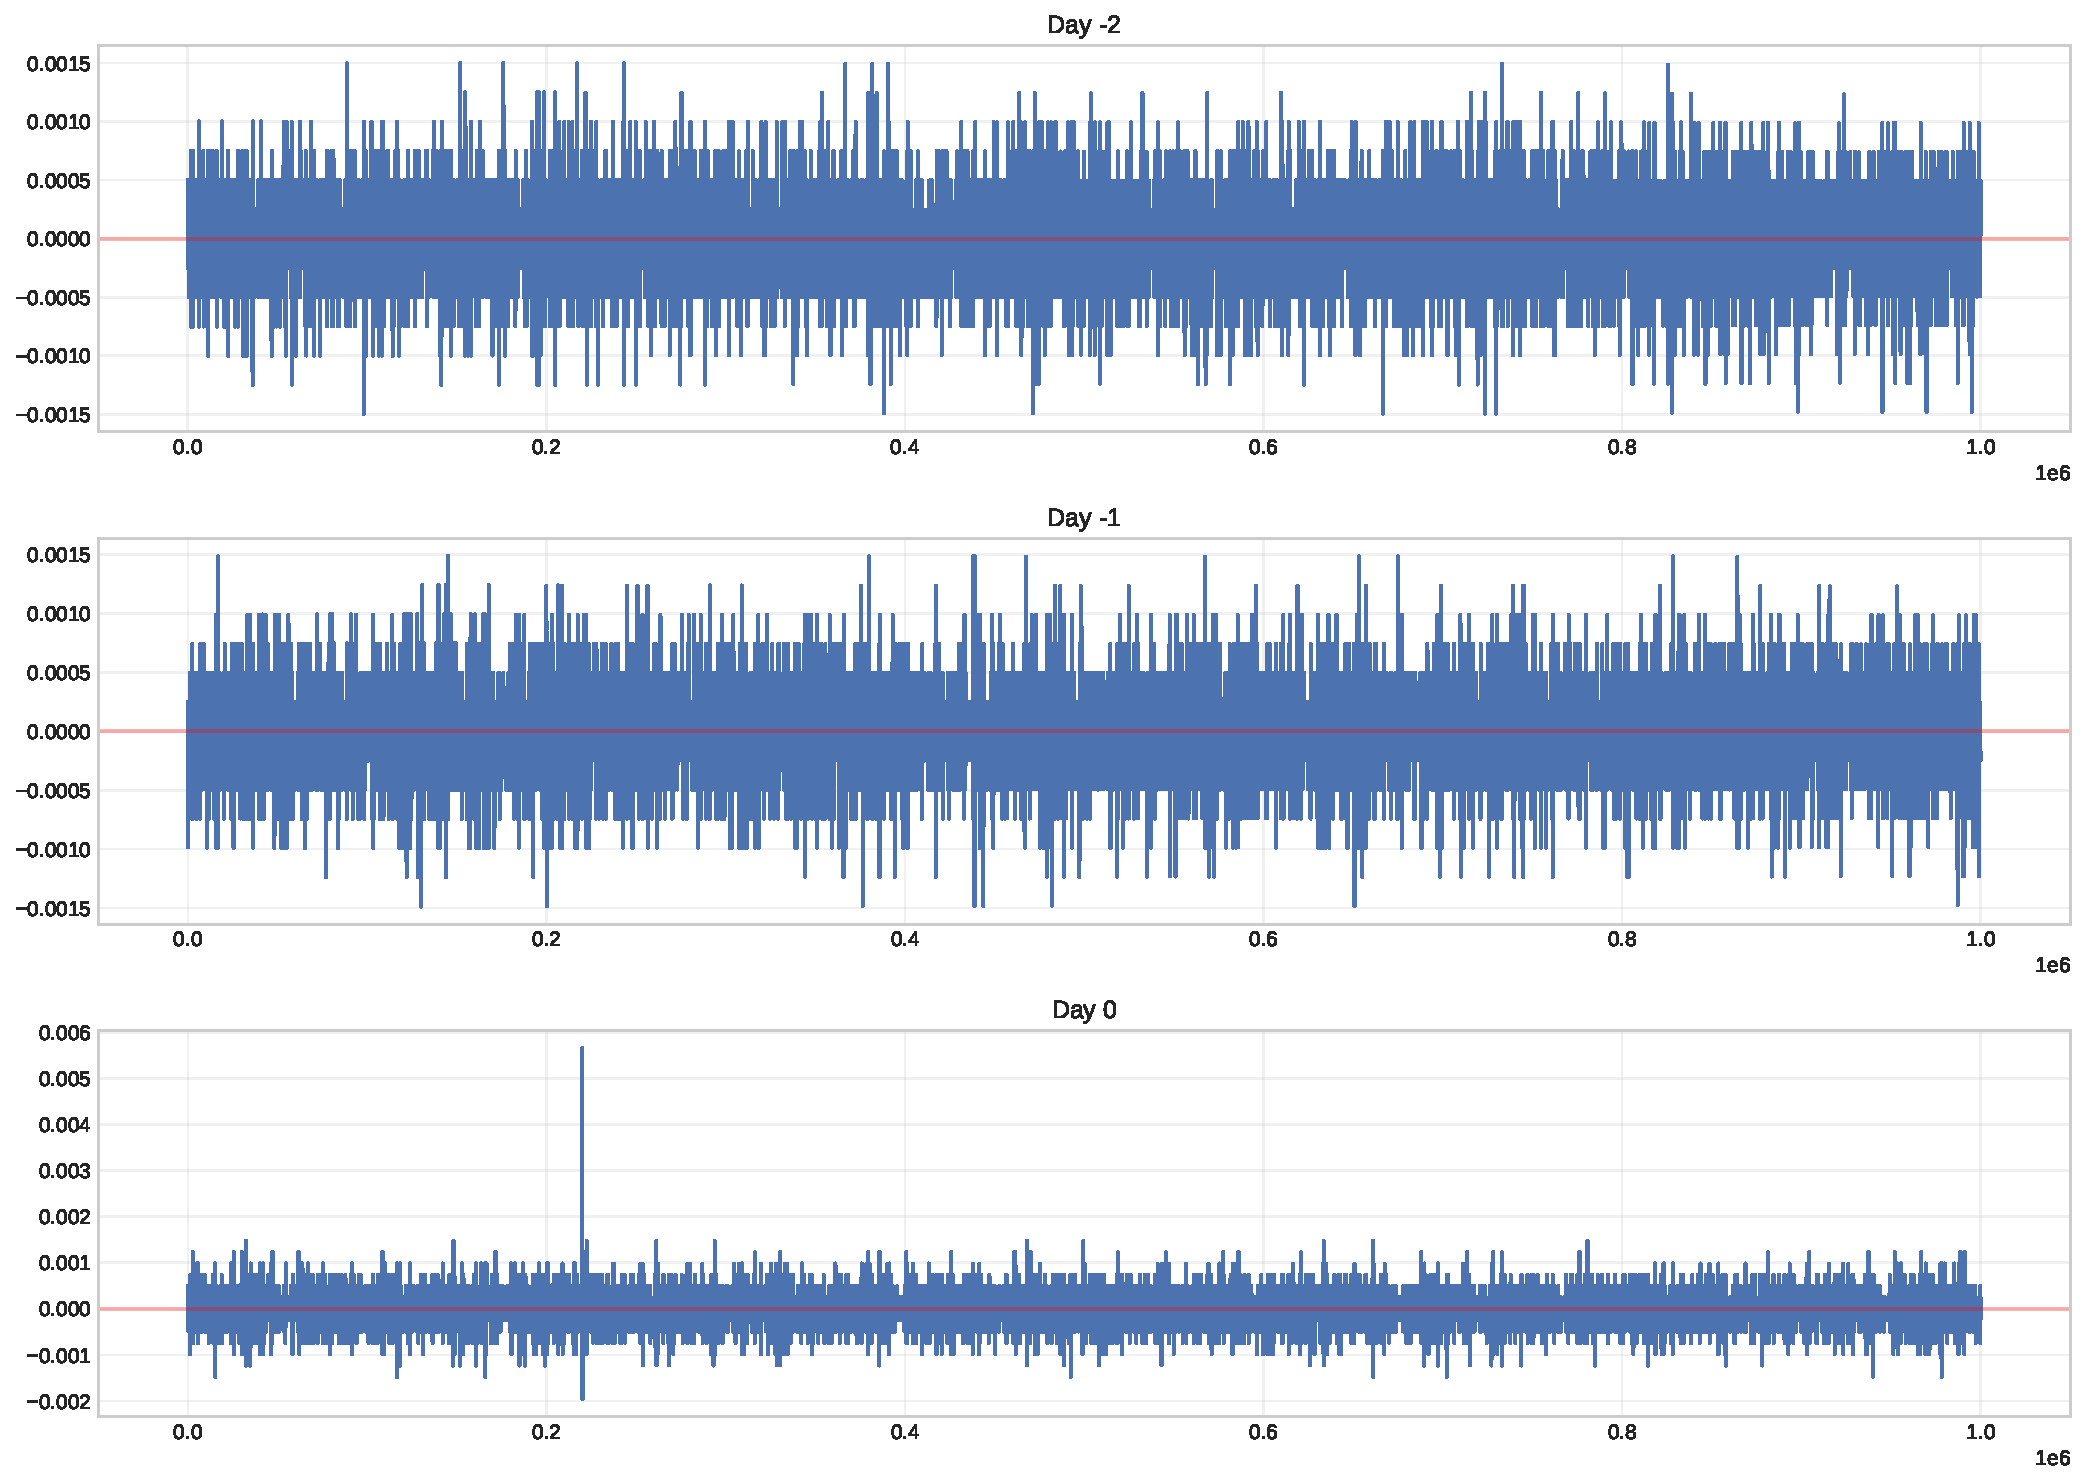
\includegraphics[keepaspectratio]{test_files/figure-pdf/cell-13-output-17.pdf}}

\pandocbounded{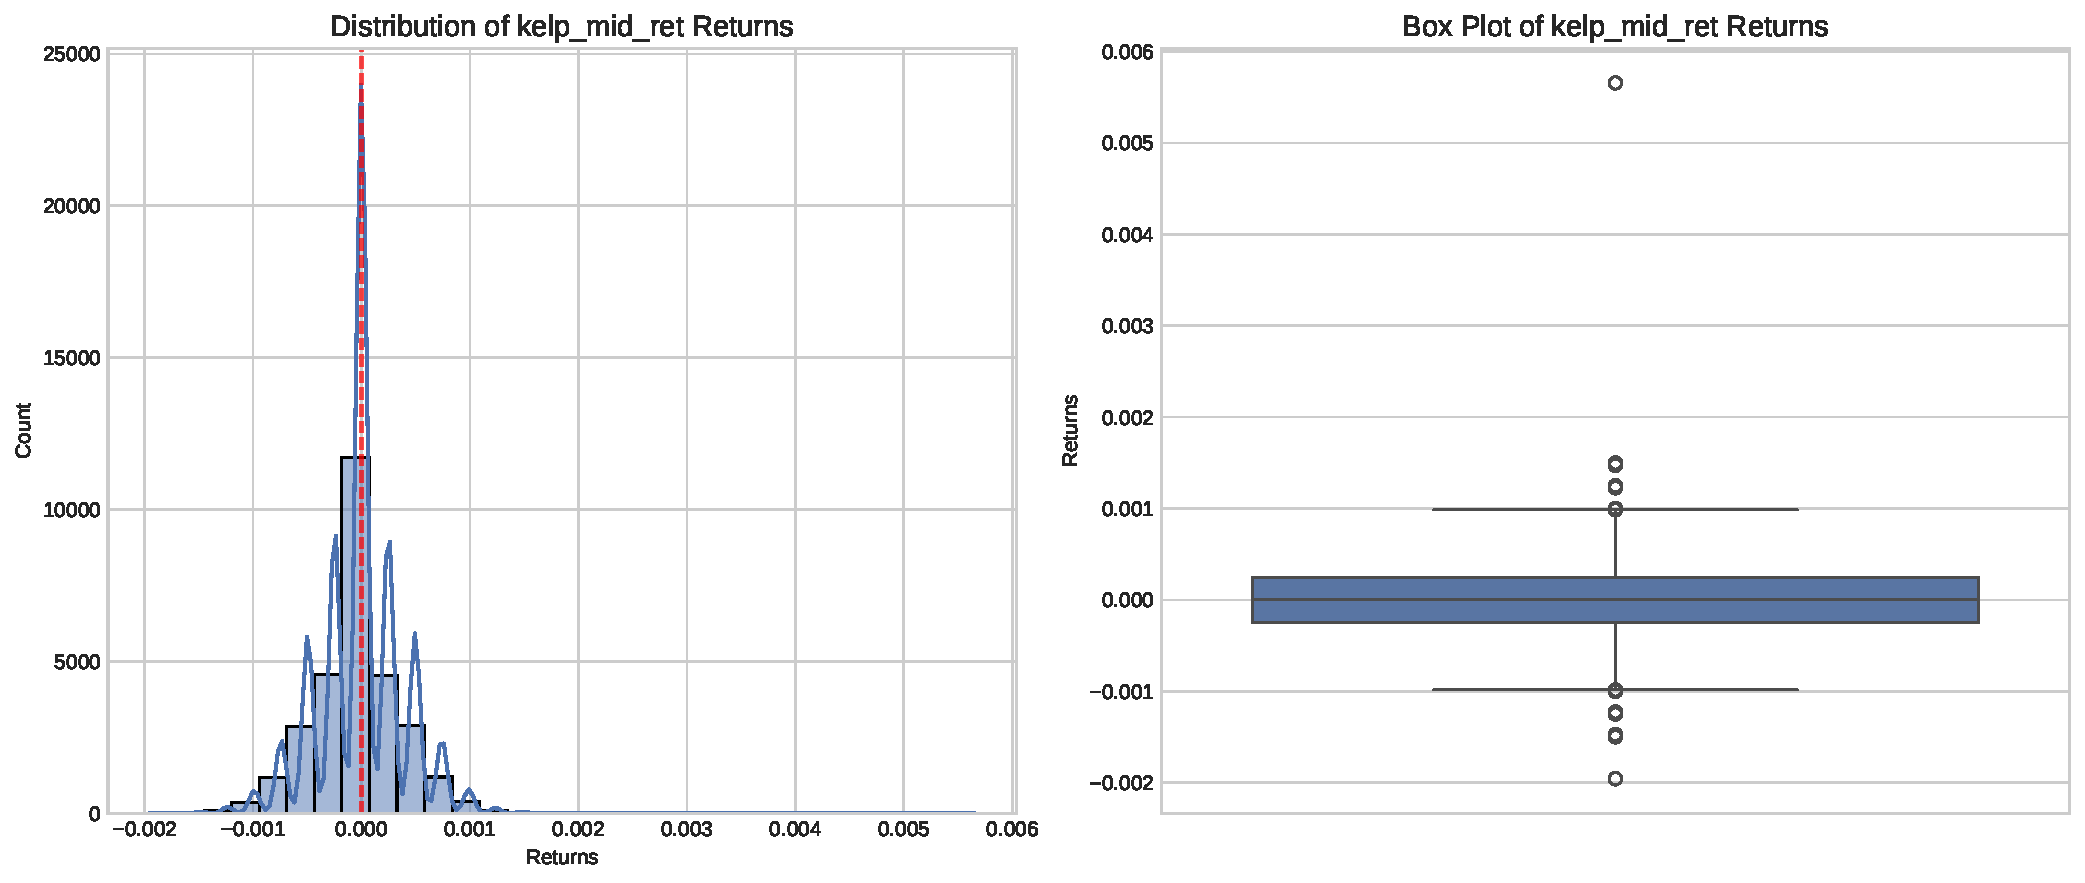
\includegraphics[keepaspectratio]{test_files/figure-pdf/cell-13-output-18.pdf}}

\begin{verbatim}
<Figure size 3000x1800 with 0 Axes>
\end{verbatim}

\pandocbounded{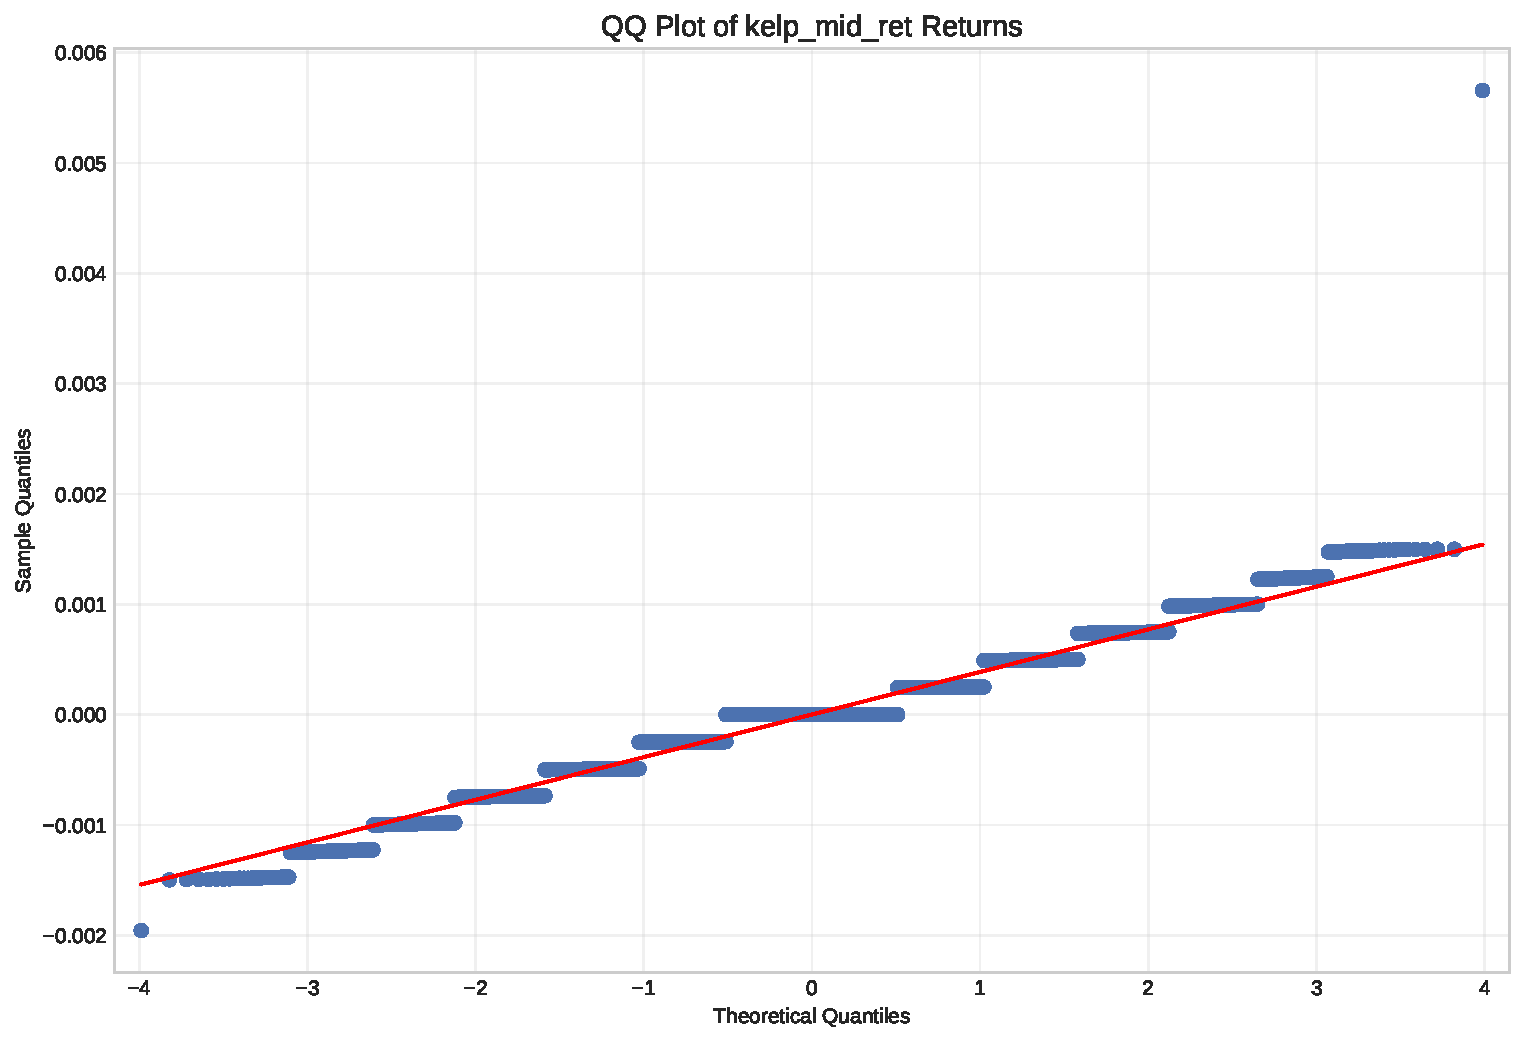
\includegraphics[keepaspectratio]{test_files/figure-pdf/cell-13-output-20.pdf}}

\begin{verbatim}
Normality Tests for kelp_mid_ret Returns:
Shapiro-Wilk Test: statistic=0.9440, p-value=0.0000
Kolmogorov-Smirnov Test: statistic=0.1957, p-value=0.0010
Anderson-Darling Test:
    15.0%: 0.576, Reject null hypothesis
    10.0%: 0.656, Reject null hypothesis
    5.0%: 0.787, Reject null hypothesis
    2.5%: 0.918, Reject null hypothesis
    1.0%: 1.092, Reject null hypothesis
\end{verbatim}

\pandocbounded{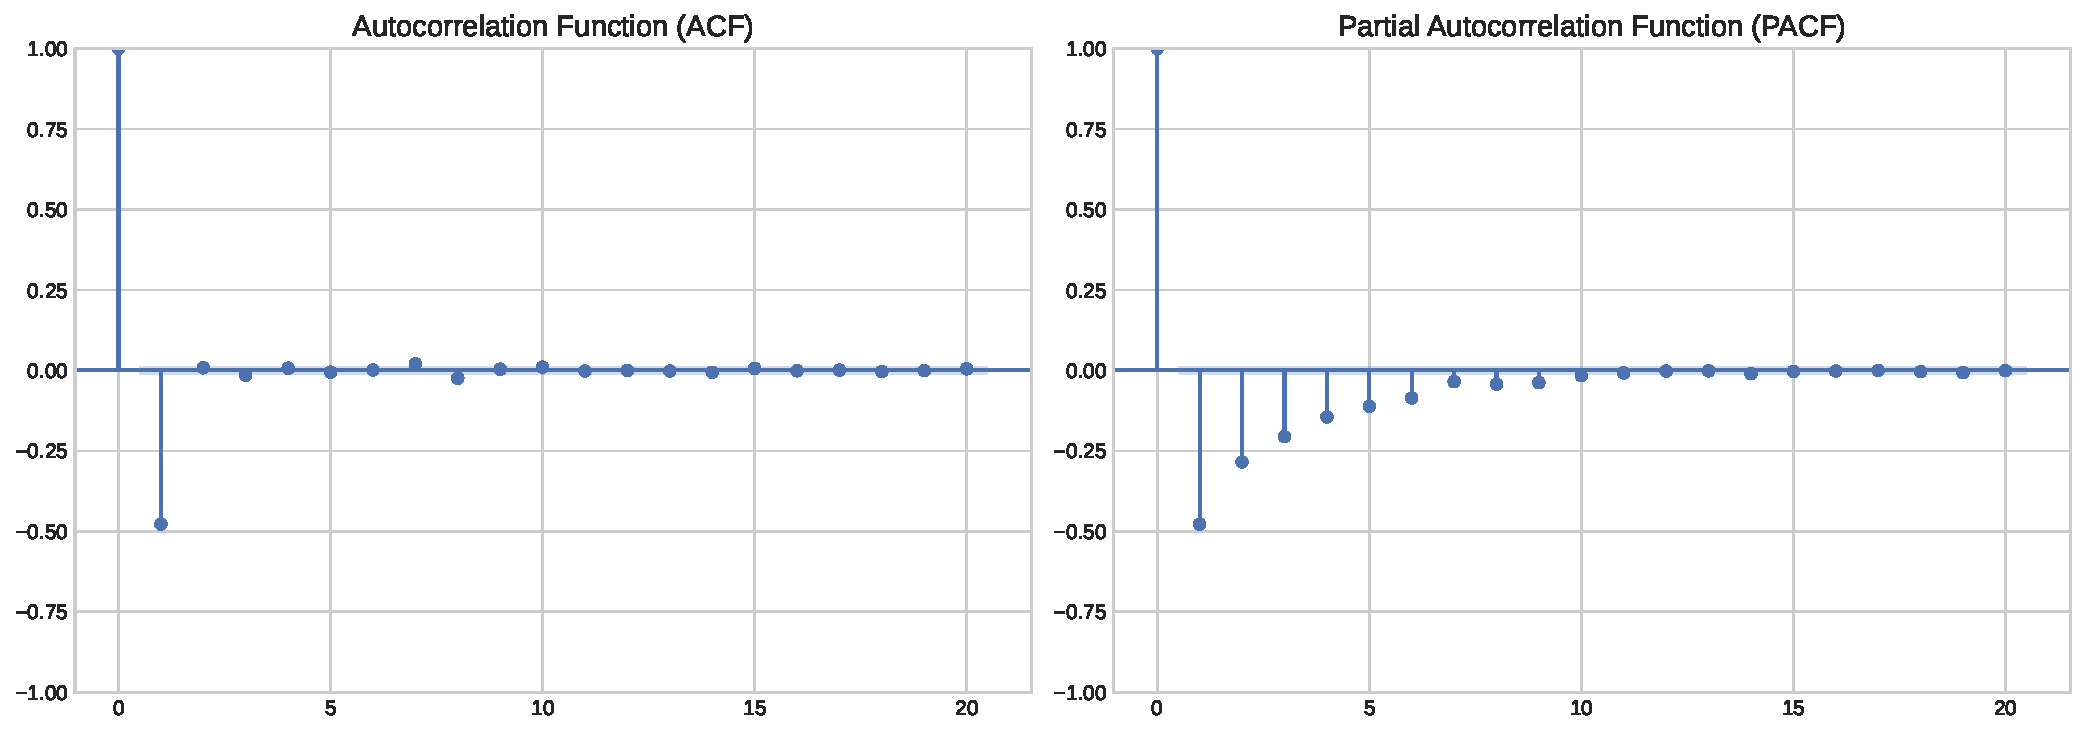
\includegraphics[keepaspectratio]{test_files/figure-pdf/cell-13-output-22.pdf}}

\pandocbounded{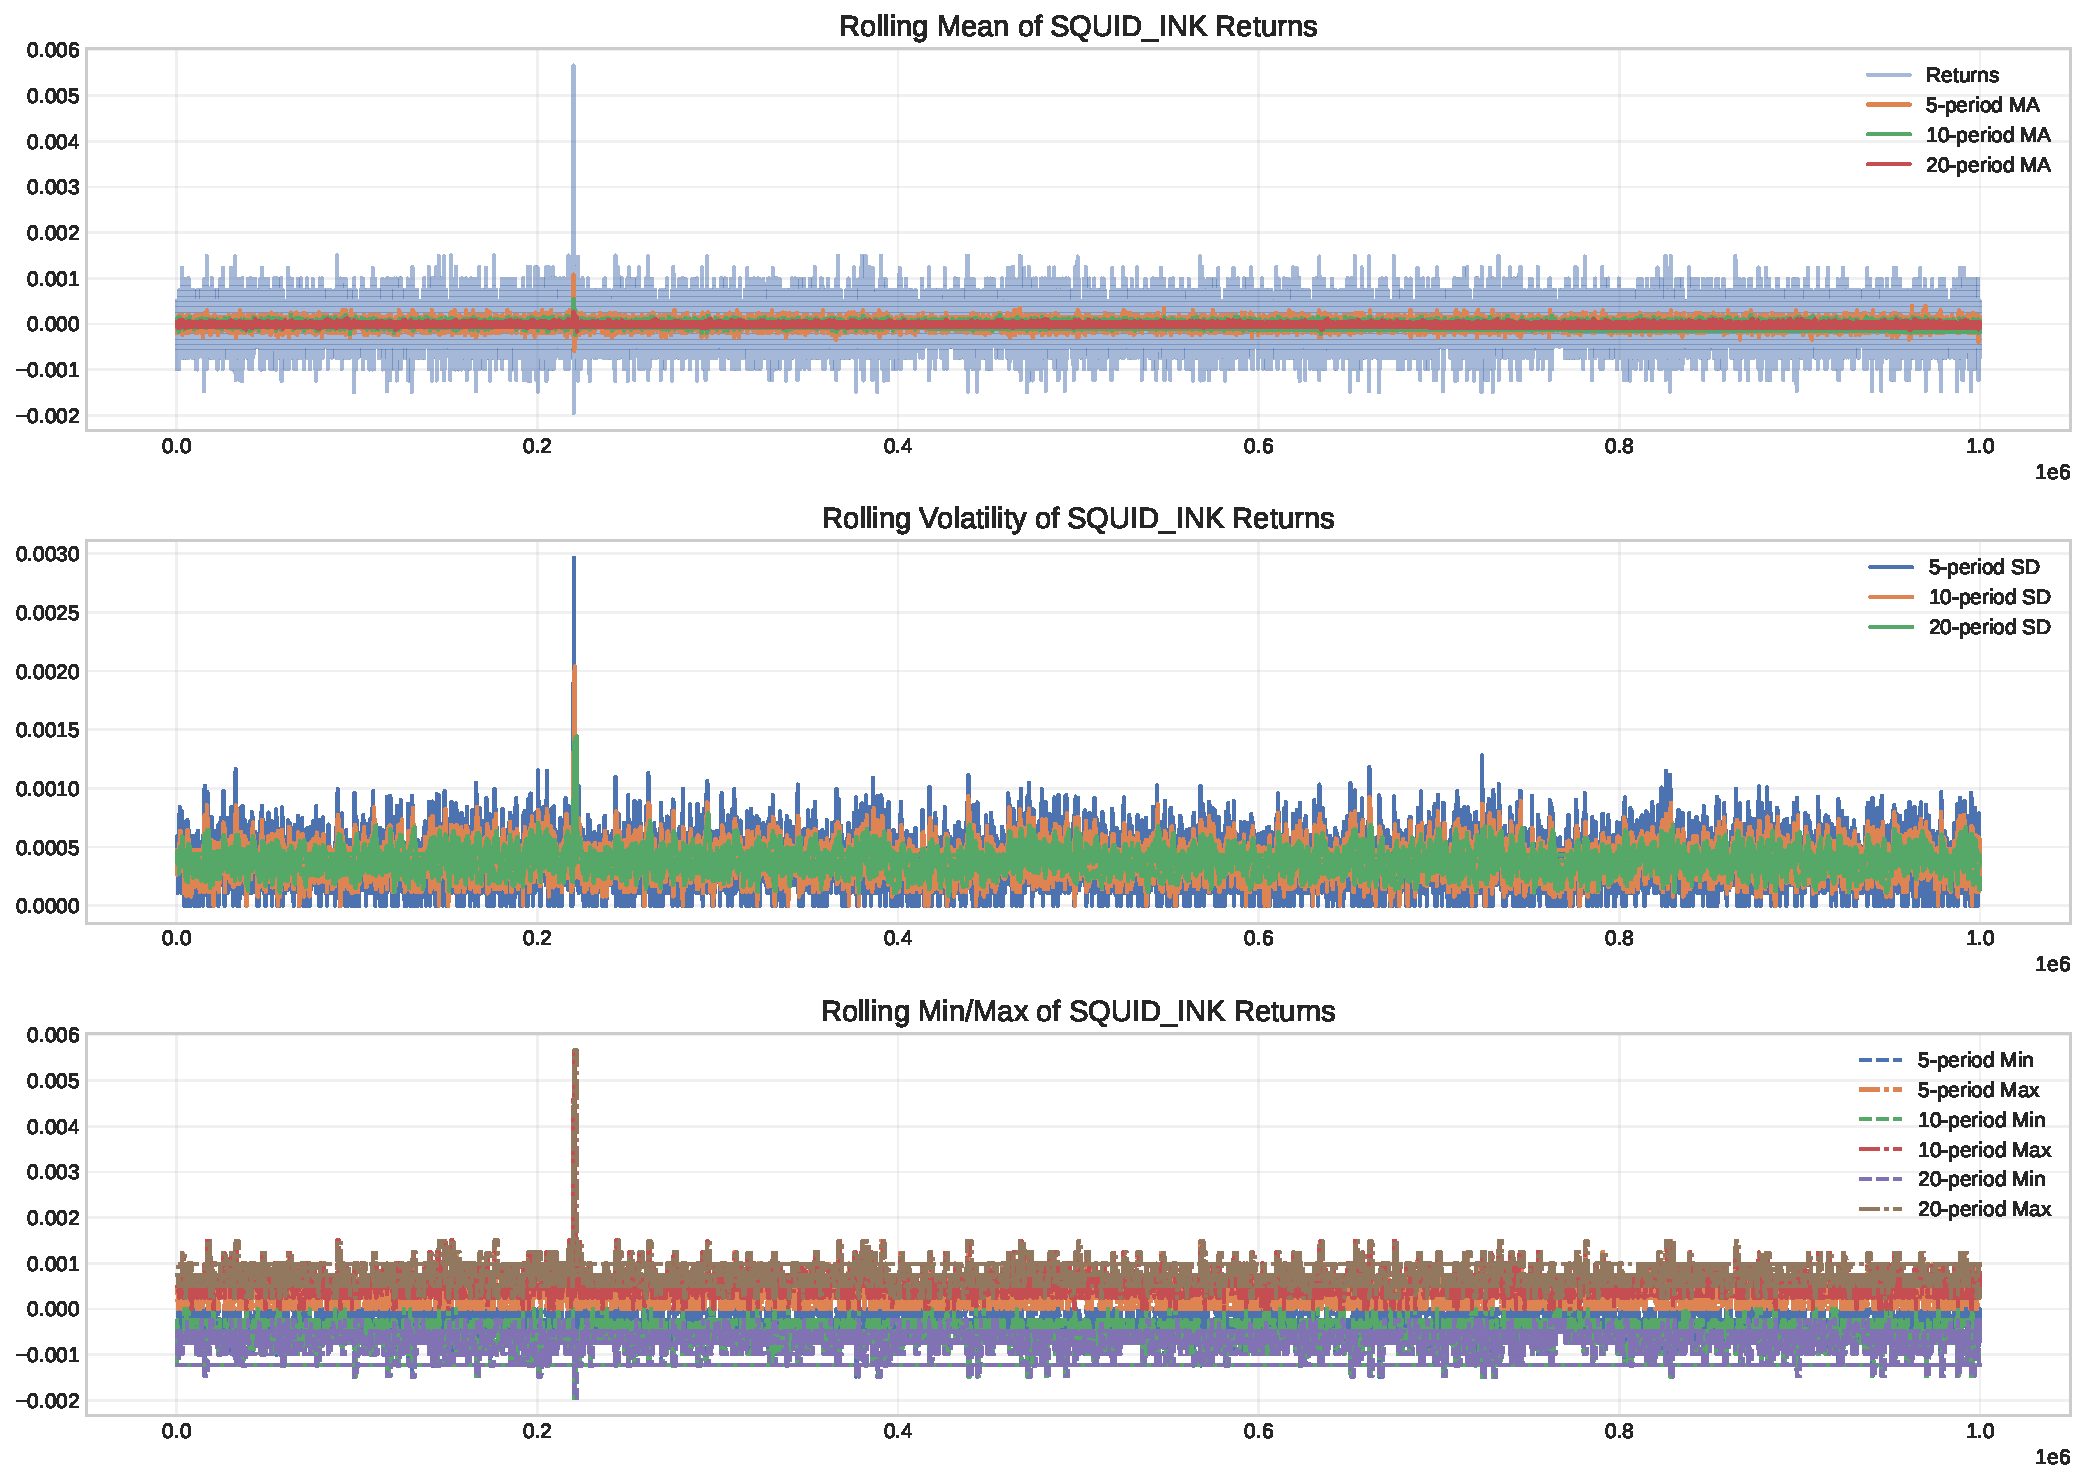
\includegraphics[keepaspectratio]{test_files/figure-pdf/cell-13-output-23.pdf}}

\pandocbounded{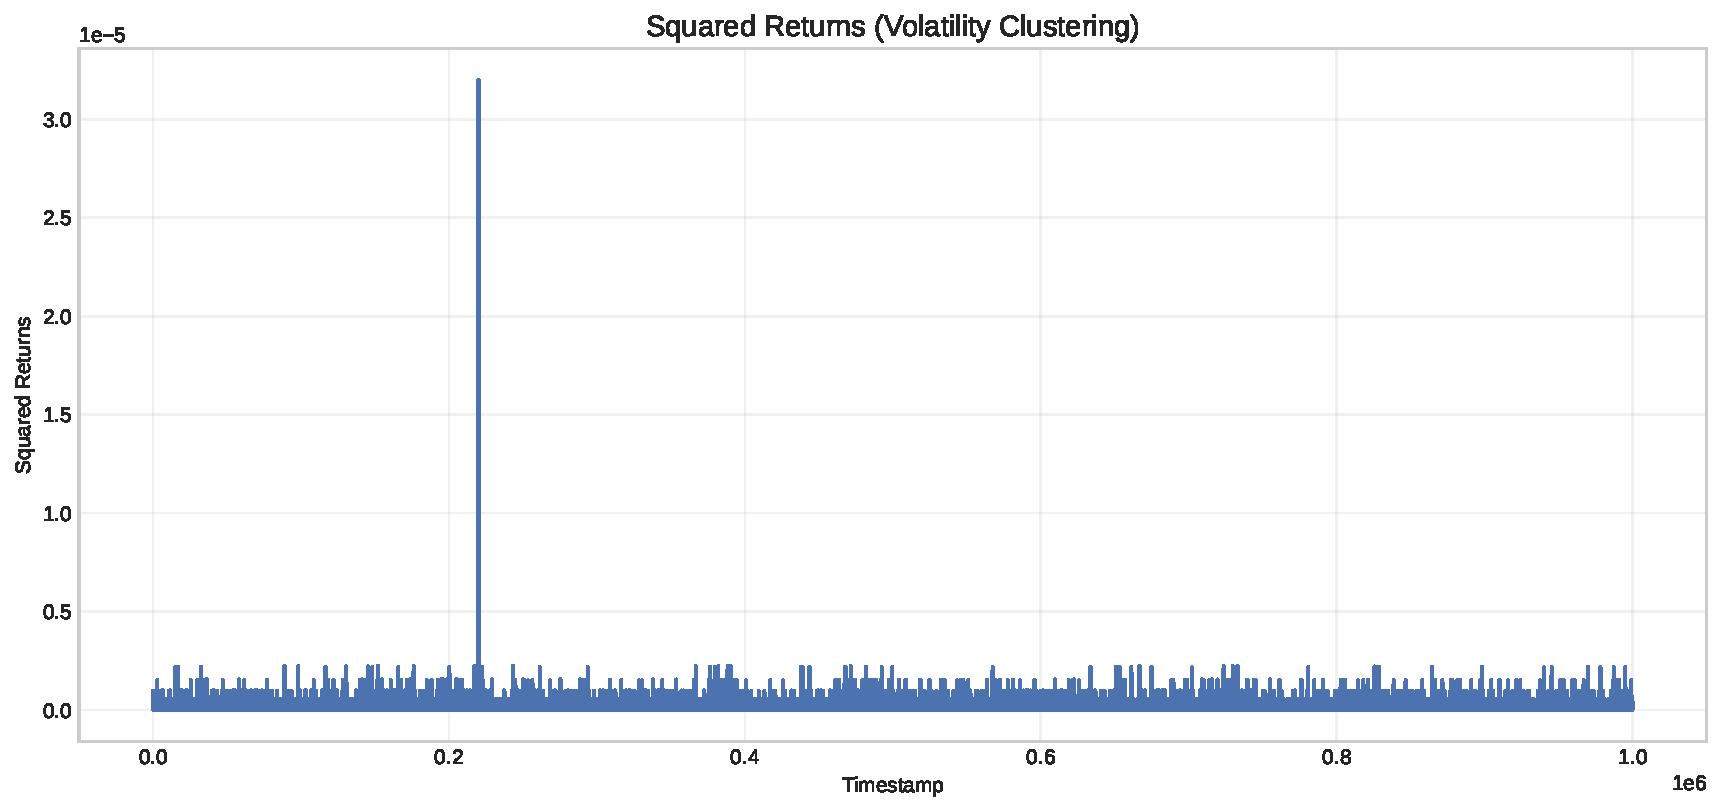
\includegraphics[keepaspectratio]{test_files/figure-pdf/cell-13-output-24.pdf}}

\pandocbounded{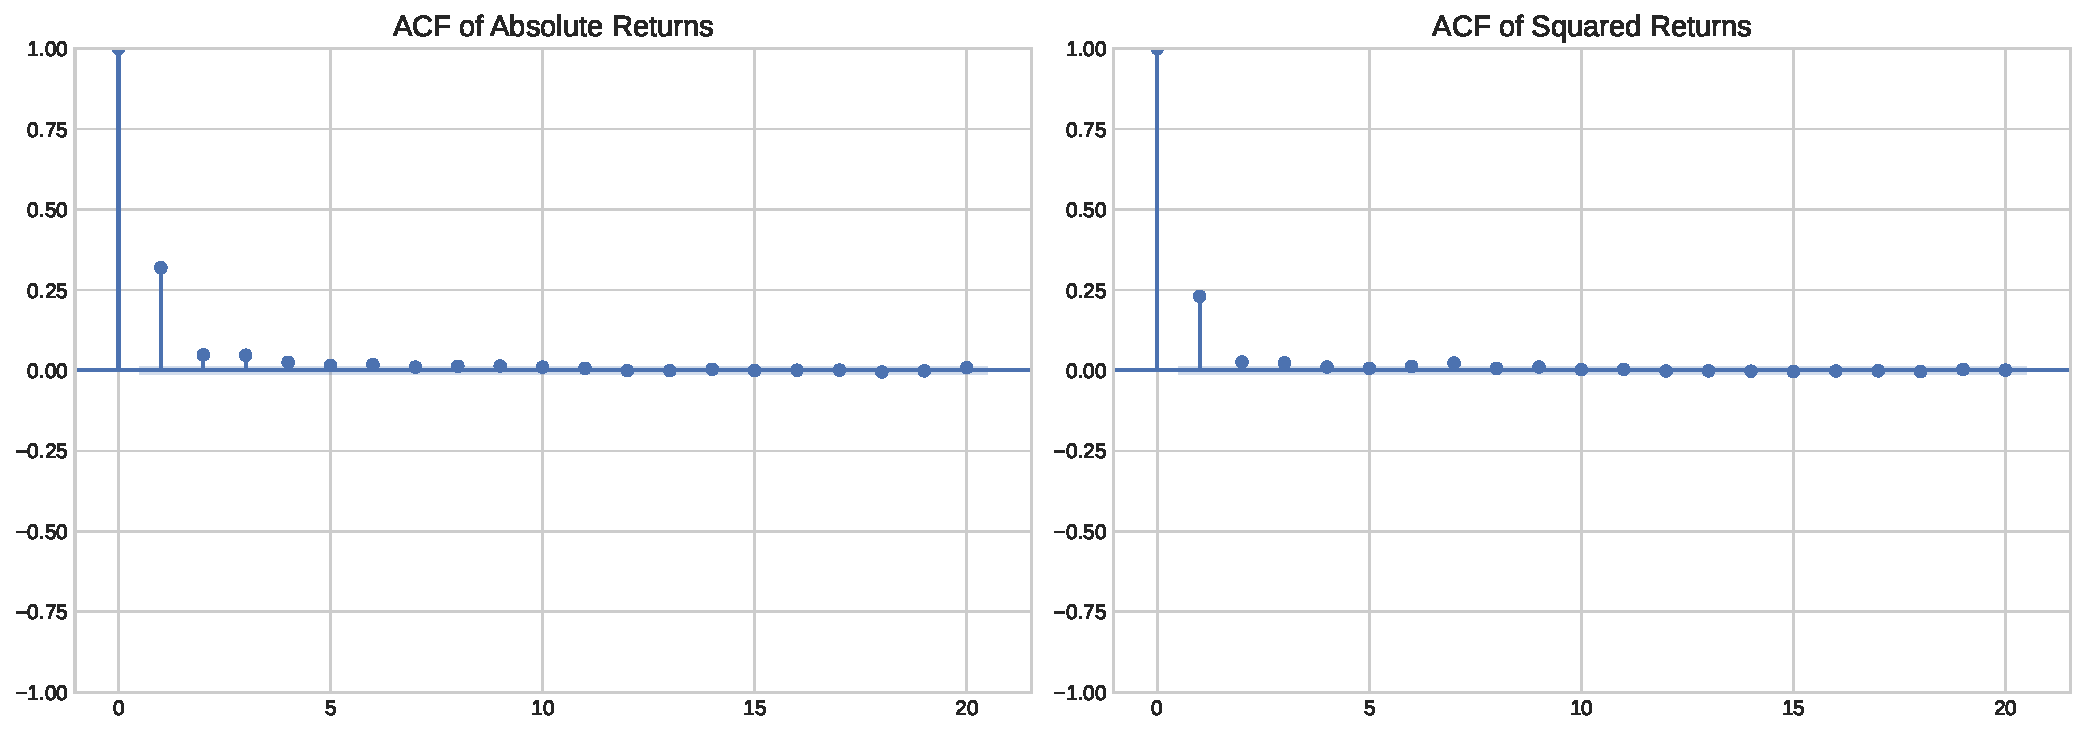
\includegraphics[keepaspectratio]{test_files/figure-pdf/cell-13-output-25.pdf}}

\pandocbounded{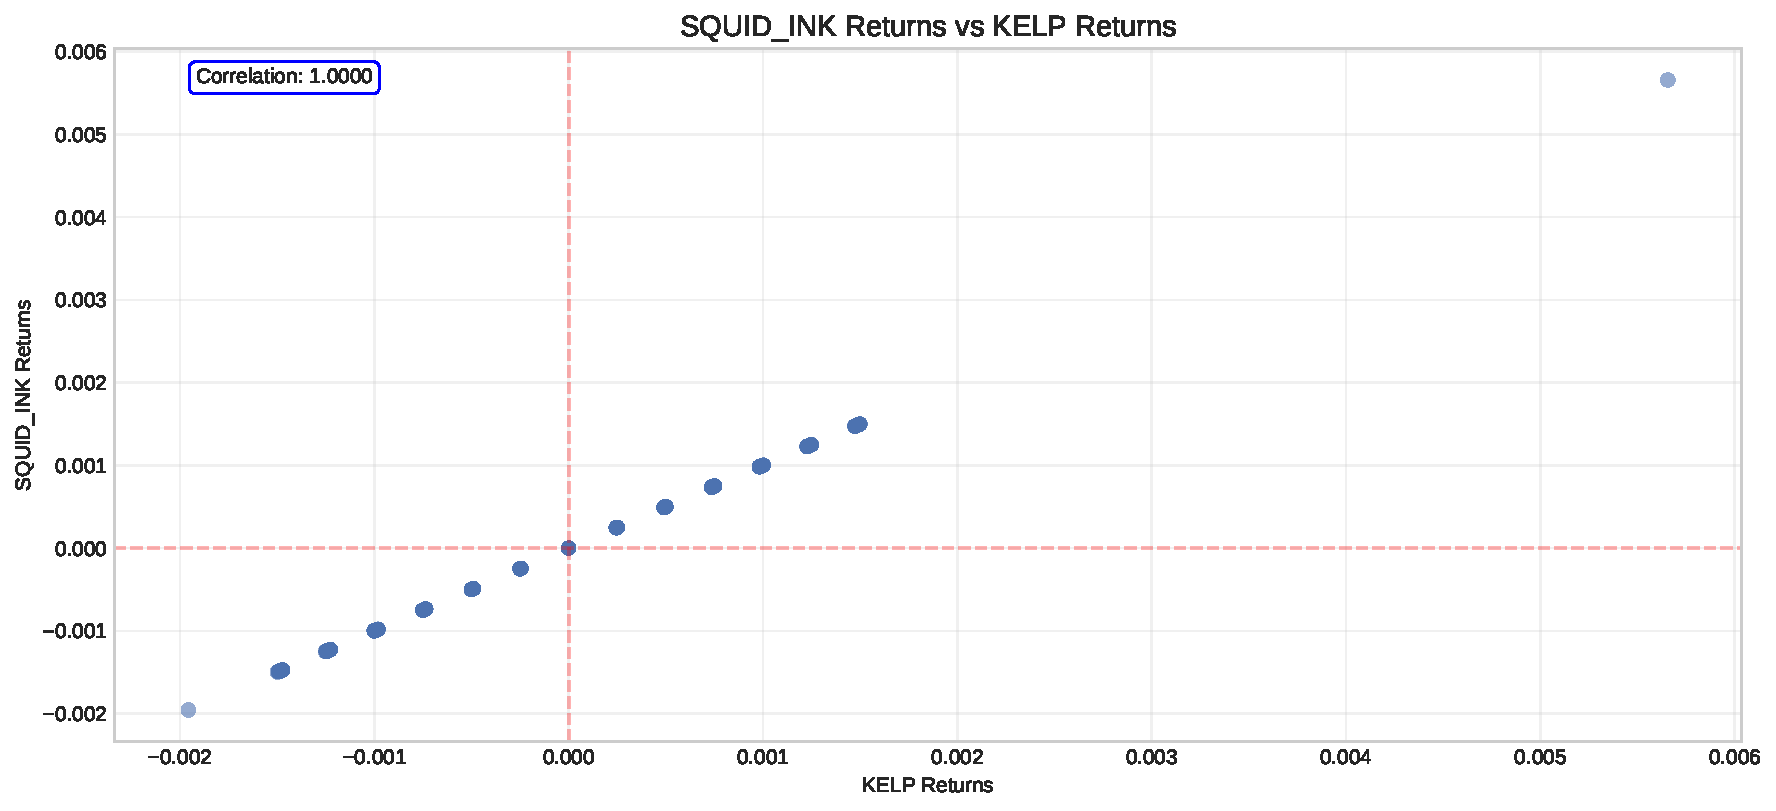
\includegraphics[keepaspectratio]{test_files/figure-pdf/cell-13-output-26.pdf}}

\pandocbounded{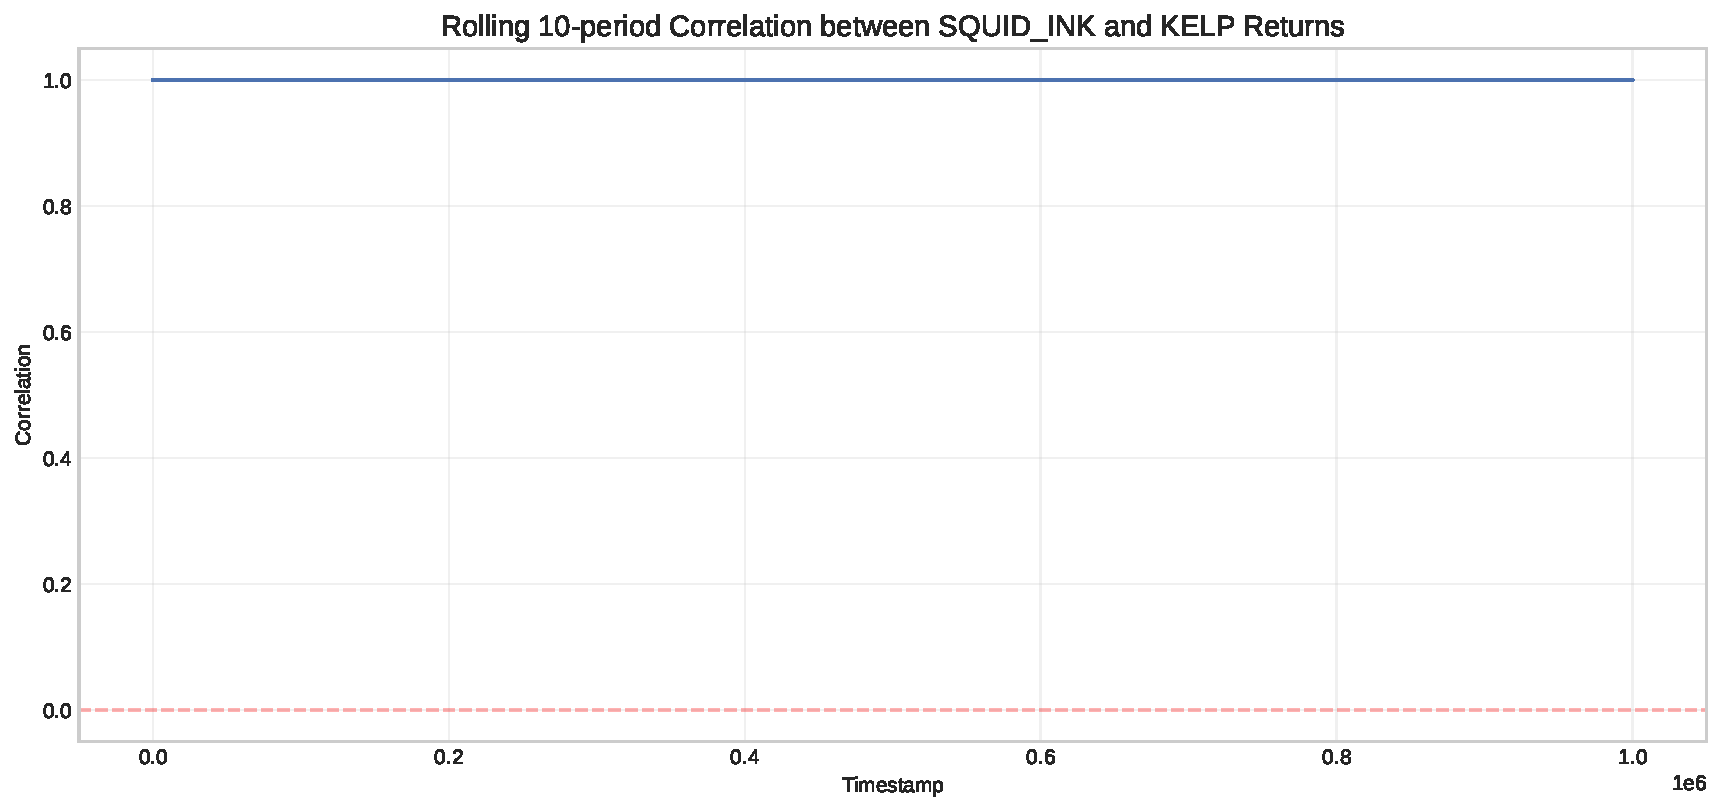
\includegraphics[keepaspectratio]{test_files/figure-pdf/cell-13-output-27.pdf}}

\pandocbounded{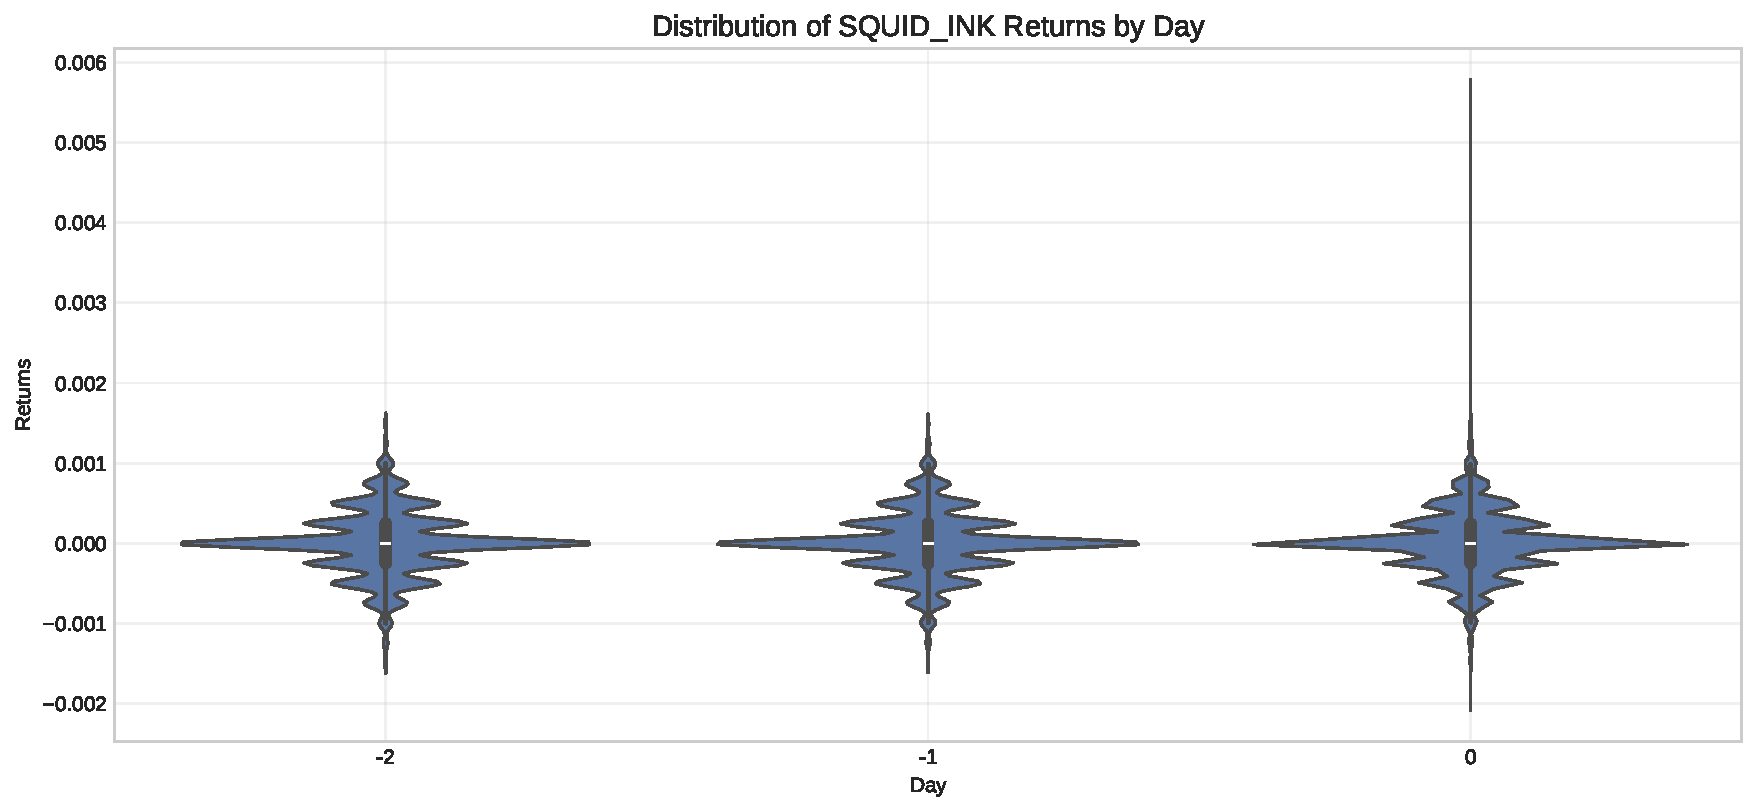
\includegraphics[keepaspectratio]{test_files/figure-pdf/cell-13-output-28.pdf}}




\end{document}
